% =====================================================================================
% AlphaAudit --- Paper 1 of the Trivijaya Quant Research programme.
%
% Every number in this paper comes from a generated macro file. Nothing is transcribed by
% hand. If a figure here disagrees with the repository, the macro file is authoritative and
% this paper is wrong.
%
%   papers/programme_numbers.tex   <- scripts/build_programme_numbers.py  (\pgm...)
%   papers/alphaaudit_numbers.tex  <- scripts/build_alphaaudit_numbers.py (\aa...)
%   papers/figures/*.png           <- scripts/build_paper_figures.py
%
% Compile: pdflatex alphaaudit && pdflatex alphaaudit   (twice, for the table of contents)
% =====================================================================================
\documentclass[11pt,a4paper]{article}

\newcommand{\paperName}{AlphaAudit}
\newcommand{\paperSubtitle}{Can an AI write a trading strategy that is\\ real, and can anything
  tell us in advance?}
\newcommand{\paperNumber}{1}
\newcommand{\paperShortHead}{Code $\rightarrow$ validity}

% =====================================================================================
% Shared style for the three papers of the Trivijaya Quant Research programme.
%
% The three papers report one programme and must look like it: same typography, same
% heading hierarchy, same table rules, same panel vocabulary, same cover structure.
% Anything paper-specific (title, running head, abstract) stays in the paper's own file.
%
% Each paper defines, BEFORE inputting this file:
%   \paperName        e.g. AlphaAudit
%   \paperSubtitle    the one-line question the paper answers
%   \paperNumber      1, 2 or 3
%   \paperShortHead   the right-hand running head
% =====================================================================================

\usepackage[utf8]{inputenc}
\usepackage[T1]{fontenc}
\usepackage{lmodern}
\usepackage[scaled=0.92]{helvet}          % sans face, headings only
\usepackage[margin=1.05in,top=1.15in,bottom=1.1in]{geometry}
\usepackage{microtype}
\usepackage{amsmath,amssymb}
\usepackage{booktabs}
\usepackage{array}
\usepackage{graphicx}
\usepackage{xcolor}
\usepackage[most]{tcolorbox}
\usepackage{titlesec}
\usepackage{enumitem}
\usepackage[font=small,labelfont={bf,color=navy},labelsep=period]{caption}
\usepackage{fancyhdr}
\usepackage{natbib}
\usepackage[colorlinks=true]{hyperref}   % loaded last, as hyperref requires

% The rupee sign is not in the default T1 encoding. A plain "Rs." is unambiguous, renders
% identically on every machine, and avoids a font dependency a reader would have to satisfy
% before they could compile the paper that asks them to check our numbers.
\providecommand{\rupee}{\textrm{Rs.}\,}

% ---- Palette: white ground, blues, one warm accent for our own errors ---------------
\definecolor{navy}{HTML}{0E2E5C}
\definecolor{steel}{HTML}{2C6BA8}
\definecolor{sky}{HTML}{5B93C7}
\definecolor{mist}{HTML}{F0F5FB}
\definecolor{ash}{HTML}{F6F7F9}
\definecolor{ink}{HTML}{1A1A1A}
\definecolor{rust}{HTML}{9C4221}

\color{ink}
\hypersetup{linkcolor=steel, citecolor=steel, urlcolor=steel}

% ---- Repository, cited often enough to deserve one definition ----------------------
\newcommand{\repourl}{https://github.com/Ashwin-aadi/Trivijaya-Quant-Research}
\newcommand{\repo}{\href{\repourl}{\texttt{github.com/Ashwin-aadi/Trivijaya-Quant-Research}}}
\newcommand{\siteurl}{https://ashwin-aadi.github.io/Trivijaya-Quant-Research/}
\newcommand{\site}{\href{\siteurl}{\texttt{ashwin-aadi.github.io/Trivijaya-Quant-Research}}}

% ---- Headings ----------------------------------------------------------------------
\newcommand{\sectionrule}{{\color{sky}\rule{\linewidth}{0.5pt}}\vspace{-0.9em}}
\titleformat{\section}[block]
  {\sffamily\large\bfseries\color{navy}}
  {\colorbox{navy}{\textcolor{white}{\sffamily\bfseries\ \thesection\ }}}{0.7em}{}
  [\vspace{0.25em}\sectionrule]
\titleformat{\subsection}[block]
  {\sffamily\normalsize\bfseries\color{navy}}{\thesubsection}{0.6em}{}
\titleformat{\paragraph}[runin]
  {\sffamily\bfseries\color{navy}}{}{0em}{}[\;]
\titlespacing*{\section}{0pt}{1.6em}{0.8em}
\titlespacing*{\subsection}{0pt}{1.2em}{0.5em}

% ---- Running head ------------------------------------------------------------------
\pagestyle{fancy}\fancyhf{}
\renewcommand{\headrulewidth}{0.4pt}
\renewcommand{\headrule}{{\color{sky}\hrule height 0.4pt}}
\fancyhead[L]{\sffamily\scriptsize\color{navy}\MakeUppercase{\paperName}}
\fancyhead[R]{\sffamily\scriptsize\color{navy}\paperShortHead}
\fancyfoot[C]{\sffamily\scriptsize\color{navy}\thepage}
\fancypagestyle{plain}{\fancyhf{}\renewcommand{\headrulewidth}{0pt}
  \fancyfoot[C]{\sffamily\scriptsize\color{navy}\thepage}}

% ---- Panels ------------------------------------------------------------------------
% A finding the reader must not skim past.
\newtcolorbox{finding}[1][]{
  enhanced, breakable, colback=mist, colframe=steel, boxrule=0pt,
  leftrule=2.5pt, arc=1pt, left=9pt, right=9pt, top=7pt, bottom=7pt,
  coltext=navy, fonttitle=\sffamily\bfseries\small, #1}

% A place where we report our own error. Deliberately a different colour from the findings,
% so a reader flipping through can see at a glance that the paper contains both.
\newtcolorbox{selfreport}[1][]{
  enhanced, breakable, colback=ash, colframe=rust, boxrule=0pt,
  leftrule=2.5pt, arc=1pt, left=9pt, right=9pt, top=7pt, bottom=7pt,
  fonttitle=\sffamily\bfseries\small, #1}

% What a result does *not* license. Every headline in this programme has one of these, because
% the distance between "we measured X on our corpus" and "X is true of AI" is where this
% literature goes wrong.
\newtcolorbox{scopebox}[1][]{
  enhanced, breakable, colback=white, colframe=sky, boxrule=0.6pt,
  arc=1pt, left=9pt, right=9pt, top=6pt, bottom=6pt,
  fonttitle=\sffamily\bfseries\small, title={\sffamily\bfseries What this does not say}, #1}

\newcommand{\keyfinding}[1]{\begin{finding}#1\end{finding}}

% A one-line takeaway that sits directly against a figure or table.
\newcommand{\takeaway}[1]{%
  \vspace{-0.4em}\noindent{\small\sffamily\color{navy}\textbf{Takeaway.}\ #1}\vspace{0.5em}}

% ---- Tables ------------------------------------------------------------------------
\newcommand{\thead}[1]{{\sffamily\bfseries\color{navy}#1}}
\renewcommand{\arraystretch}{1.15}

\setlist[itemize]{leftmargin=1.3em, itemsep=0.25em, topsep=0.4em}
\setlist[enumerate]{leftmargin=1.6em, itemsep=0.35em, topsep=0.4em}

% ---- Evidence-scope tags -----------------------------------------------------------
% The programme's central discipline: every finding is tagged with the population it was
% measured on, so a local-corpus observation can never be read as a statement about AI.
\newcommand{\tagbox}[2]{{\sffamily\scriptsize\textbf{\textcolor{#1}{[#2]}}}}
\newcommand{\taglocal}{\tagbox{steel}{LOCAL 7B}}
\newcommand{\tagfrontier}{\tagbox{navy}{FRONTIER}}
\newcommand{\tagmethod}{\tagbox{navy}{GENERATION METHOD}}
\newcommand{\tagindep}{\tagbox{rust}{GENERATOR-INDEPENDENT}}
\newcommand{\tagexpl}{\tagbox{rust}{EXPLORATORY}}
\newcommand{\tagprereg}{\tagbox{steel}{PRE-REGISTERED}}

% ---- Cover page --------------------------------------------------------------------
\newcommand{\programmecover}[1]{%
\begin{titlepage}
\thispagestyle{empty}
\raggedright
\vspace*{0.6in}
{\sffamily\small\color{steel}\MakeUppercase{Trivijaya Quant Research Programme}\\[0.2em]
 \color{sky}\rule{\linewidth}{1.2pt}}\\[0.3em]
{\sffamily\small\color{steel}Paper \paperNumber\ of 3 \quad$\cdot$\quad
 Measurement infrastructure for AI-driven quantitative research on Indian equities}

\vspace{1.5in}
{\sffamily\bfseries\color{navy}\fontsize{46}{50}\selectfont \paperName}\\[0.7em]
{\color{sky}\rule{0.4\linewidth}{2pt}}\\[0.9em]
{\sffamily\Large\color{navy} \paperSubtitle}

\vspace{0.9in}
{\sffamily\large\color{ink} Ashwin Jain}\\[0.35em]
{\rmfamily\small Department of Computer Science and Engineering\\
Motilal Nehru National Institute of Technology Allahabad\\
Prayagraj, India\\[0.2em]
\texttt{ashwinaadi2007@gmail.com}}

\vfill
{\small\sffamily\color{navy}#1}

\vspace{0.5em}
{\small\rmfamily Code, corpus, fixtures and evaluation protocol: \repo\\
Programme overview and results: \site}\\[0.6em]
{\sffamily\small\color{steel} 8 August 2026}
\end{titlepage}}

% ---- The trilogy map, printed identically in all three papers ----------------------
\newcommand{\trilogymap}{%
\begin{tcolorbox}[enhanced, colback=ash, colframe=sky, boxrule=0.6pt, arc=1pt,
  left=10pt, right=10pt, top=8pt, bottom=8pt]
\small\sffamily\color{navy}
\textbf{One programme, three questions.} Each paper answers the question the previous one
raises, on one shared universe, one shared cost model and one shared backtest engine.
\vspace{0.5em}

\begin{tabular}{@{}p{0.055\linewidth}p{0.22\linewidth}p{0.65\linewidth}@{}}
\textbf{1} & \textbf{AlphaAudit} & Can an AI produce a trading strategy that is real,
  rather than a plausible artefact of luck and leakage? \\[0.3em]
\textbf{2} & \textbf{RegimeStress} & If a strategy looks real, when does it break? \\[0.3em]
\textbf{3} & \textbf{FlowState} & If a strategy survives, how much capital can it absorb? \\
\end{tabular}
\vspace{0.4em}

\textbf{Code $\rightarrow$ validity $\rightarrow$ robustness $\rightarrow$ scale.} The
programme's overarching question is whether making the AI better makes the \emph{research}
better --- and the three papers answer it only to the extent their experiments support.
\end{tcolorbox}}

% GENERATED BY scripts/build_programme_numbers.py -- DO NOT EDIT BY HAND.
% Programme-level numbers shared by all three papers, from benchmarks/generationbench/META.json.

\newcommand{\pgmNullCorpora}{10}  % auditor_abstention_null
\newcommand{\pgmNullCombos}{70}  % auditor_abstention_null
\newcommand{\pgmNullBeating}{0}  % auditor_abstention_null
\newcommand{\pgmScaffoldArms}{5}  % compute-matched control
\newcommand{\pgmScaffoldWins}{0}  % compute-matched control
\newcommand{\pgmLocalExec}{40.7}  % G1 funnel
\newcommand{\pgmLocalTrade}{14.6}  % G1 funnel
\newcommand{\pgmLocalHoldMed}{-0.616}  % G1 holdout
\newcommand{\pgmClaudeTrade}{100.0}  % frontier funnel
\newcommand{\pgmGPTTrade}{100.0}  % frontier funnel
\newcommand{\pgmGeminiTrade}{100.0}  % frontier funnel
\newcommand{\pgmClaudeExec}{100.0}  % frontier funnel
\newcommand{\pgmGPTExec}{100.0}  % frontier funnel
\newcommand{\pgmGeminiExec}{100.0}  % frontier funnel
\newcommand{\pgmClaudeHoldMed}{-0.770}  % frontier holdout
\newcommand{\pgmGPTHoldMed}{-1.149}  % frontier holdout
\newcommand{\pgmGeminiHoldMed}{-1.149}  % frontier holdout
\newcommand{\pgmPlainDraws}{830}  % paradigm funnel
\newcommand{\pgmPlainExec}{40.7}  % paradigm funnel
\newcommand{\pgmPlainTrade}{14.6}  % paradigm funnel
\newcommand{\pgmPlainSurv}{8.6}  % funnel.json
\newcommand{\pgmPlainDevMed}{0.366}  % paradigm backtests
\newcommand{\pgmPlainHoldMed}{-0.616}  % paradigm holdout
\newcommand{\pgmPlainHoldPos}{27.6}  % paradigm holdout
\newcommand{\pgmPlainTrials}{844}  % trial ledger
\newcommand{\pgmPlainPbo}{0.114}  % audit_results
\newcommand{\pgmPlainKnife}{17.4}  % calibration
\newcommand{\pgmPlainFrag}{0.539}  % tier-2 stress
\newcommand{\pgmPlainFragN}{101}  % tier-2 stress
\newcommand{\pgmPlainCapMed}{2.60}  % capacity, deployed
\newcommand{\pgmPlainCapMax}{23.65}  % capacity, deployed
\newcommand{\pgmPlainCapN}{115}  % capacity, deployed
\newcommand{\pgmPlainNearCash}{6}  % exposure
\newcommand{\pgmPlainRedund}{13.0}  % redundancy
\newcommand{\pgmPlainPZero}{0.0}  % redundancy power
\newcommand{\pgmPlainXArm}{13.9}  % cross-arm duplicates
\newcommand{\pgmPlainK}{--}  % RULE 11 control
\newcommand{\pgmPlainCtrlYield}{--}  % RULE 11 control
\newcommand{\pgmPlainTreatYield}{--}  % RULE 11 control
\newcommand{\pgmPlainAuapBest}{-1.3754}  % ablation
\newcommand{\pgmPlainAuapN}{121}  % ablation
\newcommand{\pgmCotDraws}{800}  % paradigm funnel
\newcommand{\pgmCotExec}{36.8}  % paradigm funnel
\newcommand{\pgmCotTrade}{11.5}  % paradigm funnel
\newcommand{\pgmCotSurv}{8.0}  % funnel.json
\newcommand{\pgmCotDevMed}{0.449}  % paradigm backtests
\newcommand{\pgmCotHoldMed}{-0.051}  % paradigm holdout
\newcommand{\pgmCotHoldPos}{47.9}  % paradigm holdout
\newcommand{\pgmCotTrials}{811}  % trial ledger
\newcommand{\pgmCotPbo}{0.162}  % audit_results
\newcommand{\pgmCotKnife}{3.7}  % calibration
\newcommand{\pgmCotFrag}{0.615}  % tier-2 stress
\newcommand{\pgmCotFragN}{89}  % tier-2 stress
\newcommand{\pgmCotCapMed}{1.77}  % capacity, deployed
\newcommand{\pgmCotCapMax}{61.35}  % capacity, deployed
\newcommand{\pgmCotCapN}{84}  % capacity, deployed
\newcommand{\pgmCotNearCash}{8}  % exposure
\newcommand{\pgmCotRedund}{17.3}  % redundancy
\newcommand{\pgmCotPZero}{0.2}  % redundancy power
\newcommand{\pgmCotXArm}{19.8}  % cross-arm duplicates
\newcommand{\pgmCotK}{2}  % RULE 11 control
\newcommand{\pgmCotCtrlYield}{27.1}  % RULE 11 control
\newcommand{\pgmCotTreatYield}{11.5}  % RULE 11 control
\newcommand{\pgmCotAuapBest}{-1.6264}  % ablation
\newcommand{\pgmCotAuapN}{92}  % ablation
\newcommand{\pgmPlanDraws}{365}  % paradigm funnel
\newcommand{\pgmPlanExec}{22.7}  % paradigm funnel
\newcommand{\pgmPlanTrade}{6.8}  % paradigm funnel
\newcommand{\pgmPlanSurv}{5.5}  % funnel.json
\newcommand{\pgmPlanDevMed}{0.768}  % paradigm backtests
\newcommand{\pgmPlanHoldMed}{-0.060}  % paradigm holdout
\newcommand{\pgmPlanHoldPos}{48.3}  % paradigm holdout
\newcommand{\pgmPlanTrials}{370}  % trial ledger
\newcommand{\pgmPlanPbo}{0.139}  % audit_results
\newcommand{\pgmPlanKnife}{4.3}  % calibration
\newcommand{\pgmPlanFrag}{0.523}  % tier-2 stress
\newcommand{\pgmPlanFragN}{24}  % tier-2 stress
\newcommand{\pgmPlanCapMed}{3.85}  % capacity, deployed
\newcommand{\pgmPlanCapMax}{36.88}  % capacity, deployed
\newcommand{\pgmPlanCapN}{25}  % capacity, deployed
\newcommand{\pgmPlanNearCash}{0}  % exposure
\newcommand{\pgmPlanRedund}{0.0}  % redundancy
\newcommand{\pgmPlanPZero}{61.2}  % redundancy power
\newcommand{\pgmPlanXArm}{13.0}  % cross-arm duplicates
\newcommand{\pgmPlanK}{3}  % RULE 11 control
\newcommand{\pgmPlanCtrlYield}{39.1}  % RULE 11 control
\newcommand{\pgmPlanTreatYield}{6.8}  % RULE 11 control
\newcommand{\pgmPlanAuapBest}{-0.6056}  % ablation
\newcommand{\pgmPlanAuapN}{25}  % ablation
\newcommand{\pgmReflectDraws}{288}  % paradigm funnel
\newcommand{\pgmReflectExec}{34.0}  % paradigm funnel
\newcommand{\pgmReflectTrade}{10.1}  % paradigm funnel
\newcommand{\pgmReflectSurv}{6.2}  % funnel.json
\newcommand{\pgmReflectDevMed}{-0.589}  % paradigm backtests
\newcommand{\pgmReflectHoldMed}{-1.151}  % paradigm holdout
\newcommand{\pgmReflectHoldPos}{6.5}  % paradigm holdout
\newcommand{\pgmReflectTrials}{582}  % trial ledger
\newcommand{\pgmReflectPbo}{0.090}  % audit_results
\newcommand{\pgmReflectKnife}{32.0}  % calibration
\newcommand{\pgmReflectFrag}{1.035}  % tier-2 stress
\newcommand{\pgmReflectFragN}{21}  % tier-2 stress
\newcommand{\pgmReflectCapMed}{1.38}  % capacity, deployed
\newcommand{\pgmReflectCapMax}{9.86}  % capacity, deployed
\newcommand{\pgmReflectCapN}{25}  % capacity, deployed
\newcommand{\pgmReflectNearCash}{4}  % exposure
\newcommand{\pgmReflectRedund}{8.0}  % redundancy
\newcommand{\pgmReflectPZero}{55.9}  % redundancy power
\newcommand{\pgmReflectXArm}{24.0}  % cross-arm duplicates
\newcommand{\pgmReflectK}{3}  % RULE 11 control
\newcommand{\pgmReflectCtrlYield}{39.1}  % RULE 11 control
\newcommand{\pgmReflectTreatYield}{10.1}  % RULE 11 control
\newcommand{\pgmReflectAuapBest}{-1.4013}  % ablation
\newcommand{\pgmReflectAuapN}{29}  % ablation
\newcommand{\pgmGraphDraws}{152}  % paradigm funnel
\newcommand{\pgmGraphExec}{29.6}  % paradigm funnel
\newcommand{\pgmGraphTrade}{8.6}  % paradigm funnel
\newcommand{\pgmGraphSurv}{5.3}  % funnel.json
\newcommand{\pgmGraphDevMed}{0.108}  % paradigm backtests
\newcommand{\pgmGraphHoldMed}{-0.507}  % paradigm holdout
\newcommand{\pgmGraphHoldPos}{28.6}  % paradigm holdout
\newcommand{\pgmGraphTrials}{156}  % trial ledger
\newcommand{\pgmGraphPbo}{0.104}  % audit_results
\newcommand{\pgmGraphKnife}{8.3}  % calibration
\newcommand{\pgmGraphFrag}{0.430}  % tier-2 stress
\newcommand{\pgmGraphFragN}{12}  % tier-2 stress
\newcommand{\pgmGraphCapMed}{9.91}  % capacity, deployed
\newcommand{\pgmGraphCapMax}{36.88}  % capacity, deployed
\newcommand{\pgmGraphCapN}{11}  % capacity, deployed
\newcommand{\pgmGraphNearCash}{2}  % exposure
\newcommand{\pgmGraphRedund}{0.0}  % redundancy
\newcommand{\pgmGraphPZero}{88.0}  % redundancy power
\newcommand{\pgmGraphXArm}{0.0}  % cross-arm duplicates
\newcommand{\pgmGraphK}{6}  % RULE 11 control
\newcommand{\pgmGraphCtrlYield}{64.3}  % RULE 11 control
\newcommand{\pgmGraphTreatYield}{8.6}  % RULE 11 control
\newcommand{\pgmGraphAuapBest}{-1.0880}  % ablation
\newcommand{\pgmGraphAuapN}{13}  % ablation
\newcommand{\pgmMctsDraws}{60}  % paradigm funnel
\newcommand{\pgmMctsExec}{98.3}  % paradigm funnel
\newcommand{\pgmMctsTrade}{58.3}  % paradigm funnel
\newcommand{\pgmMctsSurv}{43.3}  % funnel.json
\newcommand{\pgmMctsDevMed}{0.750}  % paradigm backtests
\newcommand{\pgmMctsHoldMed}{0.047}  % paradigm holdout
\newcommand{\pgmMctsHoldPos}{60.0}  % paradigm holdout
\newcommand{\pgmMctsTrials}{736}  % trial ledger
\newcommand{\pgmMctsPbo}{0.179}  % audit_results
\newcommand{\pgmMctsKnife}{8.6}  % calibration
\newcommand{\pgmMctsFrag}{0.615}  % tier-2 stress
\newcommand{\pgmMctsFragN}{32}  % tier-2 stress
\newcommand{\pgmMctsCapMed}{5.16}  % capacity, deployed
\newcommand{\pgmMctsCapMax}{36.88}  % capacity, deployed
\newcommand{\pgmMctsCapN}{33}  % capacity, deployed
\newcommand{\pgmMctsNearCash}{2}  % exposure
\newcommand{\pgmMctsRedund}{14.3}  % redundancy
\newcommand{\pgmMctsPZero}{31.5}  % redundancy power
\newcommand{\pgmMctsXArm}{5.7}  % cross-arm duplicates
\newcommand{\pgmMctsK}{14}  % RULE 11 control
\newcommand{\pgmMctsCtrlYield}{89.1}  % RULE 11 control
\newcommand{\pgmMctsTreatYield}{58.3}  % RULE 11 control
\newcommand{\pgmMctsAuapBest}{0.0124}  % ablation
\newcommand{\pgmMctsAuapN}{35}  % ablation
\newcommand{\pgmPooledTrials}{3,499}  % pooled trial ledger
\newcommand{\pgmParadigmDraws}{2,495}  % sum of paradigm draws
\newcommand{\pgmParadigmArms}{6}  % methodology axis

% GENERATED BY scripts/build_alphaaudit_numbers.py -- DO NOT EDIT BY HAND.
% Covers the generator-validation section only. The rest of the AlphaAudit paper
% predates this pipeline and still states its figures inline; that is a known gap.

\newcommand{\aaGvArms}{3}  % generator_validation.json
\newcommand{\aaGvAuapBeats}{0}  % ablation_holdout.json
\newcommand{\aaGvAuapCells}{21}  % ablation_holdout.json
\newcommand{\aaGvBar}{0.95}  % generator_validation.json
\newcommand{\aaGvClaudeAuapBest}{-0.6083}  % ablation_holdout.json
\newcommand{\aaGvClaudeAuapLayers}{semantic}  % ablation_holdout.json
\newcommand{\aaGvClaudeBestGross}{1.0685}  % frontier_gap_measures.json
\newcommand{\aaGvClaudeBestNet}{0.7990}  % frontier_gap_measures.json
\newcommand{\aaGvClaudeCostDrop}{0.5795}  % frontier_gap_measures.json
\newcommand{\aaGvClaudeDevSharpe}{-0.1635}  % generator_validation.json
\newcommand{\aaGvClaudeExecuted}{20}  % generator_validation.json
\newcommand{\aaGvClaudeFlips}{1}  % frontier_gap_measures.json
\newcommand{\aaGvClaudeHoldBest}{+0.4419}  % generator_validation.json
\newcommand{\aaGvClaudeHoldSharpe}{-0.5781}  % generator_validation.json
\newcommand{\aaGvClaudeN}{20}  % generator_validation.json
\newcommand{\aaGvClaudePbo}{0.0378}  % generator_validation.json
\newcommand{\aaGvClaudeRandomHigh}{-0.3004}  % ablation_holdout.json
\newcommand{\aaGvClaudeRandomLow}{-0.8711}  % ablation_holdout.json
\newcommand{\aaGvClaudeSemantic}{6}  % generator_validation.json
\newcommand{\aaGvClaudeStatic}{0}  % generator_validation.json
\newcommand{\aaGvClaudeStatistical}{20}  % generator_validation.json
\newcommand{\aaGvClearedDev}{0}  % generator_validation.json
\newcommand{\aaGvClearedHoldout}{0}  % generator_validation.json
\newcommand{\aaGvFlipsTotal}{11}  % frontier_gap_measures.json
\newcommand{\aaGvGeminiAuapBest}{-1.7411}  % ablation_holdout.json
\newcommand{\aaGvGeminiAuapLayers}{static}  % ablation_holdout.json
\newcommand{\aaGvGeminiBestGross}{1.0952}  % frontier_gap_measures.json
\newcommand{\aaGvGeminiBestNet}{0.9315}  % frontier_gap_measures.json
\newcommand{\aaGvGeminiCostDrop}{0.8120}  % frontier_gap_measures.json
\newcommand{\aaGvGeminiDevSharpe}{-0.5854}  % generator_validation.json
\newcommand{\aaGvGeminiExecuted}{20}  % generator_validation.json
\newcommand{\aaGvGeminiFlips}{4}  % frontier_gap_measures.json
\newcommand{\aaGvGeminiHoldBest}{+0.3827}  % generator_validation.json
\newcommand{\aaGvGeminiHoldSharpe}{-1.4768}  % generator_validation.json
\newcommand{\aaGvGeminiN}{20}  % generator_validation.json
\newcommand{\aaGvGeminiPbo}{0.0037}  % generator_validation.json
\newcommand{\aaGvGeminiRandomHigh}{-0.8580}  % ablation_holdout.json
\newcommand{\aaGvGeminiRandomLow}{-2.2476}  % ablation_holdout.json
\newcommand{\aaGvGeminiSemantic}{5}  % generator_validation.json
\newcommand{\aaGvGeminiStatic}{1}  % generator_validation.json
\newcommand{\aaGvGeminiStatistical}{20}  % generator_validation.json
\newcommand{\aaGvGptAuapBest}{-0.9717}  % ablation_holdout.json
\newcommand{\aaGvGptAuapLayers}{semantic}  % ablation_holdout.json
\newcommand{\aaGvGptBestGross}{1.0773}  % frontier_gap_measures.json
\newcommand{\aaGvGptBestNet}{0.8016}  % frontier_gap_measures.json
\newcommand{\aaGvGptCostDrop}{0.5004}  % frontier_gap_measures.json
\newcommand{\aaGvGptDevSharpe}{-0.1394}  % generator_validation.json
\newcommand{\aaGvGptExecuted}{20}  % generator_validation.json
\newcommand{\aaGvGptFlips}{6}  % frontier_gap_measures.json
\newcommand{\aaGvGptHoldBest}{+0.3376}  % generator_validation.json
\newcommand{\aaGvGptHoldSharpe}{-0.9491}  % generator_validation.json
\newcommand{\aaGvGptN}{20}  % generator_validation.json
\newcommand{\aaGvGptPbo}{0.0190}  % generator_validation.json
\newcommand{\aaGvGptRandomHigh}{-0.5319}  % ablation_holdout.json
\newcommand{\aaGvGptRandomLow}{-1.4806}  % ablation_holdout.json
\newcommand{\aaGvGptSemantic}{2}  % generator_validation.json
\newcommand{\aaGvGptStatic}{0}  % generator_validation.json
\newcommand{\aaGvGptStatistical}{20}  % generator_validation.json
\newcommand{\aaGvMatchedDevLarge}{3}  % generator_validation.json
\newcommand{\aaGvMatchedDevSmall}{41}  % generator_validation.json
\newcommand{\aaGvMatchedHoldoutLarge}{0}  % generator_validation.json
\newcommand{\aaGvMatchedHoldoutSmall}{0}  % generator_validation.json
\newcommand{\aaGvNLarge}{20}  % generator_validation.json
\newcommand{\aaGvNSmall}{5}  % generator_validation.json
\newcommand{\aaGvRequestsPerArm}{4}  % generator_validation.json
\newcommand{\aaGvStaticTotal}{1}  % generator_validation.json
\newcommand{\aaGvSubsamples}{1000}  % generator_validation.json
\newcommand{\aaGvTotal}{60}  % generator_validation.json
\newcommand{\aaLocalAuapBest}{-1.1967}  % runs/pooled/ablation_holdout.json
\newcommand{\aaLocalAuapLayers}{semantic}  % runs/pooled/ablation_holdout.json
\newcommand{\aaLocalCostDrop}{0.5867}  % runs/pooled/gross_vs_net.json
\newcommand{\aaLocalDraws}{1550}  % runs/pooled/audit_results.json
\newcommand{\aaLocalFlips}{35}  % runs/pooled/gross_vs_net.json
\newcommand{\aaLocalFlipsOf}{225}  % runs/pooled/gross_vs_net.json
\newcommand{\aaLocalFlipsPct}{15.6}  % runs/pooled/gross_vs_net.json
\newcommand{\aaLocalHoldoutN}{225}  % runs/pooled/holdout_results.json
\newcommand{\aaLocalHoldoutSharpe}{-1.0351}  % runs/pooled/holdout_results.json
\newcommand{\aaLocalRandomHigh}{-0.8600}  % runs/pooled/ablation_holdout.json
\newcommand{\aaLocalRandomLow}{-1.2208}  % runs/pooled/ablation_holdout.json
\newcommand{\aaLocalRankable}{225}  % runs/pooled/backtest_results.json
\newcommand{\aaLocalRankablePct}{14.5}  % runs/pooled/backtest_results.json
\newcommand{\aaLocalStatic}{222}  % runs/pooled/audit_results.json
\newcommand{\aaLocalStaticPct}{14.3}  % runs/pooled/audit_results.json
\newcommand{\aaLocalStaticRankable}{28}  % runs/pooled/audit_results.json
\newcommand{\aaLocalStaticRankablePct}{12.4}  % runs/pooled/audit_results.json

% GENERATED BY scripts/build_standard_factor_comparison.py -- DO NOT EDIT BY HAND.
% The standard-factor arm, on every frozen test, for both papers.

\newcommand{\sfN}{11}  % control set
\newcommand{\sfStatic}{0}  % positive_control
\newcommand{\sfFlipped}{2}  % positive_control
\newcommand{\sfRuined}{1}  % positive_control
\newcommand{\sfMedGross}{0.8239}  % positive_control
\newcommand{\sfMedNet}{0.3038}  % positive_control
\newcommand{\sfMedLost}{0.6412}  % positive_control
\newcommand{\sfCleared}{0}  % standard_factor_deflation
\newcommand{\sfMaxDsr}{0.000599}  % standard_factor_deflation
\newcommand{\sfBar}{0.95}  % standard_factor_deflation
\newcommand{\sfTrials}{11}  % PI ruling 2026-08-08
\newcommand{\sfTrialSd}{1.5461}  % standard_factor_deflation
\newcommand{\sfPbo}{0.2124}  % standard_factor_deflation
\newcommand{\sfMedFrag}{0.8581}  % tier2_fragility
\newcommand{\sfKnife}{1}  % tier2_fragility
\newcommand{\sfNondet}{0}  % regimestress calibration
\newcommand{\sfBestName}{momentum}  % highest net Sharpe in the arm
\newcommand{\sfBestNet}{0.9656}  % positive_control


% Numbers local to this paper that predate the macro pipeline are stated inline and flagged in
% Limitations. Where a quantity exists as a macro, the macro is used.

\begin{document}

% =====================================================================================
\programmecover{%
A benchmark for measuring whether machine-generated quantitative research survives
transaction costs, multiple testing and a never-touched holdout --- and whether an auditor can
tell which candidates will, before the holdout is opened.}

% =====================================================================================
\begin{abstract}
\noindent
A language model that writes trading strategies is a machine for manufacturing plausible
backtests. The two defects that make such backtests worthless --- code that secretly reads the
future, and the near-certainty that something looks brilliant if you try enough things --- are
precisely the two an ordinary evaluation cannot see. As models become better programmers, the
backtests become more plausible, not more true, and the problem gets worse rather than better.

\medskip\noindent
\textbf{We release AlphaAudit: an environment, a protocol and a corpus for measuring whether
machine-written trading research is real.} It comprises a survivorship-free point-in-time
universe of Indian equities, a transaction-cost model built to the Indian statutory schedule and
verified against a broker's public calculator, deliberately-cheating and honest fixture suites, a
hash-chained trial ledger the generator cannot write to, a frozen one-shot evaluation protocol,
and \pgmParadigmDraws{} audited machine-written candidates.

\medskip\noindent
\textbf{What we measured.} Four generators --- one local 7B model and three frontier models ---
and \pgmParadigmArms{} generation methods, all issued the same frozen task specification and all
run through the same unchanged funnel. The question the programme asks is not which model writes
the best code. It is whether making the AI better makes the \emph{research} better.

\medskip\noindent
\textbf{The headline result is a separation.} On the local 7B, the binding constraint is not
cheating but competence: every draw returned parseable, interface-conforming code, and only
\pgmLocalTrade\% produced a strategy that both ran on real data and took a position. Frontier
models remove that constraint completely --- \aaGvTotal{} of \aaGvTotal{} candidates executed and
traded, a rate of 100\% against \pgmLocalTrade\%. \textbf{They do not remove the second
constraint at all.} Not one of the \aaGvTotal{} frontier candidates attained a deflated Sharpe
probability above \aaGvBar{} at its own honest trial count, on development or on holdout;
\aaGvFlipsTotal{} of them reverse the sign of their Sharpe once Indian costs are charged; and
across ten independently generated corpora and \pgmNullCombos{} auditor configurations,
\pgmNullBeating{} beat random rejection at matched coverage out of sample.

\medskip\noindent
\textbf{Better code did not become better evidence.} We report that as the benchmark's first
entry rather than as a result to be improved upon: the environment, the protocol and the
fixtures are independent of whether our auditor worked, and a stronger auditor can contest the
second claim against exactly the same apparatus.
\end{abstract}

\vspace{0.2em}
\noindent{\small\sffamily\color{navy}\textbf{Keywords:} backtest overfitting \textbullet\
deflated Sharpe ratio \textbullet\ lookahead bias \textbullet\ selective prediction \textbullet\
LLM code generation \textbullet\ transaction costs \textbullet\ Indian equities}

% =====================================================================================
\section*{Key findings}
\addcontentsline{toc}{section}{Key findings}

Each of the six numbers below answers a question. Every one carries the sample it was measured
on, and every one is tagged with the population it describes --- because the distance between
\emph{``we observed this in our corpus''} and \emph{``AI does this''} is where this literature
usually goes wrong.

\begin{finding}[title={1.\ \ Does the AI cheat, or does it simply not work? \hfill\taglocal}]
\textbf{It does not work.} All 1{,}550 local draws returned syntactically valid, interface-conforming
Python with a stated rationale --- a 100\% success rate at looking correct. Only 631 (\pgmLocalExec\%)
survived contact with real data, and of those 406 (64.3\%) never took a position.
\textbf{\pgmLocalTrade\% of the corpus produced a strategy that both executes and trades.}
An auditor built to catch cheating is guarding a door most candidates never reach.
\end{finding}

\begin{finding}[title={2.\ \ Do frontier models fix that? \hfill\tagfrontier}]
\textbf{Completely.} \aaGvTotal{} of \aaGvTotal{} candidates from three frontier models executed to
completion and took a position: \textbf{100\% against the local model's \pgmLocalTrade\%.}
The execution barrier that dominates the local corpus is an artefact of model capability, and it
disappears when capability rises. Total static leak findings across all \aaGvTotal{}:
\aaGvStaticTotal{}.
\end{finding}

\begin{finding}[title={3.\ \ Does better code become better evidence? \hfill\tagfrontier\ \tagindep}]
\textbf{No.} \textbf{Zero} of \aaGvTotal{} frontier candidates cleared a deflated Sharpe
probability of \aaGvBar{} at its own trial count --- \aaGvClearedDev{} on development,
\aaGvClearedHoldout{} on the holdout --- matching the local corpus's 0 of 631. Median holdout
Sharpe is \emph{worse} for every frontier arm than for the local reference
(\pgmGPTHoldMed, \pgmClaudeHoldMed, \pgmGeminiHoldMed{} against \pgmLocalHoldMed).
\textbf{Frontier models solved the execution problem. They did not touch the evidence problem.}
\end{finding}

\begin{finding}[title={4.\ \ Are transaction costs a haircut or a filter? \hfill\taglocal\ \tagfrontier}]
\textbf{A filter.} \aaLocalFlipsPct\% of the local corpus's \aaLocalFlipsOf{} tradeable strategies
reverse the sign of their Sharpe once Indian costs are charged; none reverse the other way, as
none can; 11 are bankrupted outright. \aaGvFlipsTotal{} of \aaGvTotal{} frontier candidates flip
as well. The best surviving strategy in the corpus survives \emph{because it barely trades}, at
$2.8\times$ annual turnover. \textbf{Cost survival selects for low turnover, not for skill.}
\end{finding}

\begin{finding}[title={5.\ \ Does more elaborate prompting help? \hfill\tagmethod\ \tagprereg}]
\textbf{Not at equal compute.} Of \pgmScaffoldArms{} scaffolded generation methods ---
chain-of-thought, planning, reflection, graph-of-thoughts and Monte Carlo tree search ---
\textbf{\pgmScaffoldWins{} beat plain prompting once plain prompting was given the same token
budget} and allowed to keep its best of $k$ attempts. The scaffolding buys candidates, and the
control buys the same number of candidates more cheaply.
\end{finding}

\begin{finding}[title={6.\ \ Can the auditor tell in advance which ones are real? \hfill\tagindep}]
\textbf{Not on any corpus we generated.} Across \pgmNullCorpora{} independently generated corpora
--- six generation methods, three frontier models, and the pooled local corpus --- and all seven
combinations of the three auditor layers, \textbf{\pgmNullBeating{} of \pgmNullCombos{}
configurations beat random rejection at matched coverage on out-of-sample data.} We publish the
null rather than tune past it. It survived two subsequent corrections of our own pipeline.
\end{finding}

\vspace{0.6em}
\trilogymap

\clearpage
{\hypersetup{linkcolor=navy}\tableofcontents}
\clearpage

% =====================================================================================
\section{The question}
\label{sec:question}

A language model can now write a trading strategy. Ask one for a systematic equity strategy on
Indian large-caps and it will return a stated economic rationale, a feature specification, entry
and exit rules, position sizing, and executable code. Ask for three hundred and it will return
three hundred.

The natural next step is to backtest them, sort by Sharpe ratio, and look at the top of the list.
That procedure is worthless, and it is worthless in a way that gets \emph{worse} as the model
gets better.

\begin{finding}
The overarching question of this three-paper programme:
\textbf{does making the AI better actually make the quantitative research better?}
\smallskip

Those are two different things, and the rest of this paper exists because the literature
routinely treats them as one. \emph{Generator quality} is how well a model writes code that
compiles, runs, and does what its author intended. \emph{Research quality} is whether the
resulting finding is true. A better generator raises the first by construction. Whether it raises
the second is an empirical question, and the answer we measured is no.
\end{finding}

\subsection{Why the two come apart}

Suppose a generator improves so much that every strategy it writes executes flawlessly on the
first attempt. Nothing about that improvement makes the underlying market predictable. What it
changes is the \emph{number of plausible-looking candidates per unit of effort} --- and the
probability that the best of a large set looks impressive by luck alone rises with the size of
the set. A better generator therefore produces a better-looking best backtest and no more real
alpha. Improvement on the generator axis is improvement in the rate at which candidates arrive at
the door; it is not improvement in what is behind the door.

This is not a hypothetical worry about future models. It is the result reported here, measured on
three frontier models against a local 7B on the same task specification.

\subsection{What this paper answers, and what it does not}

AlphaAudit answers three questions and is honest about failing the fourth.

\begin{enumerate}
\item \textbf{Where do machine-written strategies actually die?} Not where the literature
assumes. \S\ref{sec:local}.
\item \textbf{Does a more capable generator change that?} Yes at the front of the funnel,
not at all at the back. \S\ref{sec:frontier}.
\item \textbf{Does a more elaborate generation \emph{method} change it?} Not at equal
compute. \S\ref{sec:methods}.
\item \textbf{Can an auditor identify the survivors in advance?} \textbf{We could not build
one that does}, on any of ten corpora. \S\ref{sec:null}.
\end{enumerate}

The fourth is the one we set out to answer positively, and the null is reported at the same
prominence as the rest. A benchmark whose reference implementation fails is still a benchmark;
what would destroy it is adjusting the implementation until it passed.

% =====================================================================================
\section{What can go wrong with an AI-generated strategy}
\label{sec:whatgoeswrong}

Before any machinery, the failure modes --- in plain terms, because the rest of the paper is
about detecting them and a reader who has not met them cannot judge whether the detectors are
adequate.

\subsection{The code reads the future}

A backtest simulates trading through history. It is trivially easy, and usually accidental, to
write one that uses information from after the moment it claims to be deciding. A signal computed
from today's closing price cannot be used to buy at today's opening price, but nothing in ordinary
Python stops you writing that. The resulting equity curve is not a slightly optimistic estimate
--- it is a measurement of a machine that can see tomorrow, and it can be arbitrarily good.

This is called \textbf{lookahead bias} or \textbf{leakage}. It has recognisable species:

\begin{itemize}
\item \textbf{Future indexing.} Directly using a value from a later timestamp --- a
  \texttt{shift(-1)}, a reversed slice.
\item \textbf{Full-sample statistics.} Computing a mean, standard deviation or quantile over the
  whole history and using it to make decisions early in that history. The mean of a series you
  have not lived through yet is not available to you.
\item \textbf{Fitting before splitting.} Scaling features using statistics from the test period.
\item \textbf{Snooped parameters.} A lookback window or threshold chosen because it worked on the
  data being tested.
\item \textbf{Survivorship selection.} Choosing which stocks to trade in 2020 using the list of
  companies that still exist in 2025. The ones that went to zero are silently absent, and the
  strategy looks like genius rather than luck.
\end{itemize}

Only some of these announce themselves in the source. The last is a property of how the data was
assembled, not of the strategy code at all --- which is why \S\ref{sec:infra} spends as much space
on the universe as on the auditor.

\subsection{Someone tried three hundred things}

The second defect needs no bug at all. Take a market with no predictability whatsoever, generate
three hundred strategies at random, and rank them. The best will look good. Not because anything
was learned, but because the maximum of three hundred noisy numbers is large. This is
\textbf{multiple testing}, or in this setting \textbf{backtest overfitting}
\citep{bailey2017,harvey2016}.

The correction is not to shrink the winner's Sharpe ratio. It is to \emph{raise the bar} it must
clear, by the amount that luck alone would deliver given how many attempts were made
\citep{bailey2014}. With widely dispersed trials, two hundred attempts buy an expected best Sharpe
of about $2.77$ by luck --- so an observed $2.0$ from two hundred attempts is not impressive, it
is \emph{below} what chance produces.

That correction has a precondition which is where LLM pipelines quietly fail: \textbf{you must
know how many attempts were made}, honestly, including the ones that crashed, the ones you
discarded, and the ones from last week. A generator that regenerates on syntax error and reports
only its successes has destroyed the denominator. \S\ref{sec:auditor} describes the ledger we
built because of this, and \S\ref{sec:selfreport-ledger} reports the one place ours is imperfect
and why we did not repair it.

\subsection{The costs are not a rounding error}

Indian equity trading carries securities transaction tax, exchange transaction charges, an
investor protection fund levy, a SEBI turnover fee, stamp duty, GST on the brokerage and exchange
components, and a per-scrip depository charge on every sell. For a strategy that trades often,
these compound into a drag that routinely exceeds the entire apparent edge. A great many published
Indian backtests are fiction for this reason alone \citep{novymarx2016,frazzini2018}.

\subsection{The story and the code disagree}

A machine-written strategy comes with a stated rationale. Nothing enforces that the rationale
describes the code. A model can write a paragraph about liquidity provision in mid-caps and
implement momentum; it can offer a mechanism so elastic that it would explain any outcome; or it
can rediscover a forty-year-old anomaly and present it as novel. None of these is a bug --- the
code runs, the backtest is honest --- and all of them mean the finding is not what it claims.

% =====================================================================================
\section{What was available before AlphaAudit, and why it was not enough}
\label{sec:related}

Four literatures each hold part of the problem, and none holds the whole of it.

\paragraph{Code-generation benchmarks} measure whether a model writes code that passes tests
\citep{chen2021}. That is exactly the wrong success criterion here. A leaky strategy passes every
test; it is \emph{more} likely to pass, because it works better. The property we need to measure
is invisible to a test suite by construction.

\paragraph{Backtest-overfitting statistics} give us the corrections
\citep{bailey2014,bailey2017,harvey2016,lopezdeprado2018} and are the reason the statistical layer
in \S\ref{sec:auditor} is not our invention. What they do not supply is the honest denominator
when the researcher is an autonomous loop. The literature assumes a human who knows roughly how
many models they fitted.

\paragraph{Selective prediction} formalises the right question --- a system that declines to act
when unconfident is worth more than one that is occasionally brilliant and frequently wrong
\citep{elyaniv2010,geifman2017}. It has not been applied to strategy research, where the
``label'' arrives only after out-of-sample time has elapsed, and where abstention is nearly free
while a wrong action is not.

\paragraph{Finance-specific language models} \citep{wu2023} raise capability without addressing
evaluation. A more capable finance model produces more plausible candidates. Section
\ref{sec:frontier} is a direct measurement of what that does and does not buy.

\begin{finding}
The gap AlphaAudit fills: there was no environment in which a machine-written strategy corpus
could be scored for \emph{validity} --- survivorship-free, cost-realistic, trial-counted,
holdout-disciplined --- under a protocol fixed before the results were seen. Building the
environment is the contribution that does not depend on our auditor working.
\end{finding}

% =====================================================================================
\section{What we built}
\label{sec:infra}

Four components, in the order a result has to pass through them. Each is a place a published
Indian backtest commonly goes wrong.

\subsection{A universe that includes the companies that failed}

\textbf{This is the most important correctness requirement in the repository}, and getting it
wrong invalidates everything downstream regardless of the quality of the rest.

The universe on any date $t$ contains exactly the hundred most liquid NSE equities \emph{as they
were known on $t$}, including names later delisted or dropped. It is rebuilt quarterly from
exchange bhavcopy archives, ranking by median traded value over a trailing window that ends
strictly before the rebalance date. No constituent list from the present is ever applied backwards.

The verification that matters is not that the code looks right, it is that stocks actually leave:
the suite asserts the presence of at least one symbol in an early-period universe and absent from
a late one, and fails loudly otherwise. A survivorship-biased universe makes every strategy in
this paper look better than it is, and the bias is invisible in every downstream number.

\subsection{Costs at the rates in force on each trade's own date}

\texttt{src/costs/india.py} implements the Indian statutory schedule per leg, separately for
delivery and intraday, with each rate cited to its source and effective date in the docstring, and
applied \emph{as of the trade's date} rather than at today's rate. Slippage is a
volume-participation model, so cost rises with order size as a share of that day's volume; a flat
basis-point assumption was not acceptable and is not used.

The model is validated by hand-computing a \rupee 1{,}00{,}000 delivery round trip line by line
and asserting agreement to the paisa, and independently by entering the same trade into a
discount broker's public calculator. One component --- the square-root market-impact coefficient
--- remains an uncalibrated engineering assumption, and paper 3 of this programme reports the
measurement showing that daily data cannot calibrate it \citep{almgren2005}.

\subsection{An engine that raises rather than warns}

Point-in-time discipline is a property of the engine, not a convention the strategy author is
trusted to honour. Every signal carries the timestamp at which its information became available,
and the engine raises \texttt{PointInTimeError} --- an exception, not a warning --- if any order's
signal timestamp is not strictly prior to its fill timestamp. A signal computed from a session's
close may trade no earlier than the next session's open. Cross-validation is purged with an
embargo after each test fold, following \citet{lopezdeprado2018}, so overlapping label windows
cannot leak across the split.

\subsection{Fixtures: we wrote the disease before the test for it}

Three strategies in \texttt{tests/fixtures/leaky/} cheat deliberately --- one uses next-day
returns as a feature, one fits a scaler on the full sample before splitting, one selects its
universe from end-of-period membership. All three produce absurd results, which is the point:
they are the positive controls for the auditor. Thirty honest strategies --- moving-average
crossovers, simple momentum, mean reversion --- measure the false-positive rate.

\begin{scopebox}
The fixtures establish that the auditor catches cheats \emph{of the kinds we thought to write}.
They say nothing about kinds we did not. \S\ref{sec:leakclasses} reports a leak class on which
our static layer returned a zero we do not believe.
\end{scopebox}

% =====================================================================================
\section{The auditor}
\label{sec:auditor}

Three layers, each independently ablatable, so that the question ``which layer earns its place''
is answerable rather than asserted.

\subsection{$A_{\mathrm{static}}$ --- leakage by structure, not by syntax}

The static layer parses candidate source with Python's \texttt{ast} module and classifies each
finding by leak class, line number and severity. Its two strongest rules are structural rather
than syntactic: \emph{did the constructor accept bulk data?} and \emph{did the decision function
read stored state instead of the point-in-time view?} These mirror the engine's own information
boundary, which is why they catch cheats whose results look plausible. Pattern-matching
\texttt{shift(-1)} catches only the cheats that announce themselves.

Against the fixture suite the layer achieves recall $1.00$ (3 of 3 leaky) and precision $1.00$
(0 of 30 honest flagged).

\begin{selfreport}[title={This 100\% should be discounted, and here is why}]
With syntax-based detectors alone, recall was 1 of 3. The structural rules were added
\emph{after} observing that failure, and were then measured on the same three fixtures that
motivated them. That is closer to training accuracy than to a test, and we report it in the
results rather than the appendix. The genuine out-of-sample evaluation is against generated code
the detectors were never designed around (\S\ref{sec:leakclasses}), and it is far less flattering.
\end{selfreport}

\subsection{$A_{\mathrm{stat}}$ --- deflation against an honest denominator}

We compute the Deflated Sharpe Ratio of \citet{bailey2014}, which converts an observed Sharpe
$\widehat{SR}$ into the probability that it exceeds what $N$ trials would produce by luck, given
sample length $T$, skewness $\gamma_3$ and kurtosis $\gamma_4$:
\[
\mathrm{DSR} \;=\; \Phi\!\left(
\frac{(\widehat{SR} - SR_0)\sqrt{T-1}}
     {\sqrt{1 - \gamma_3 \widehat{SR} + \frac{\gamma_4 - 1}{4}\widehat{SR}^{\,2}}}
\right),
\]
where $SR_0$ is the expected maximum Sharpe across $N$ trials --- a function of both $N$ and the
\emph{dispersion} of the trials' Sharpes. Restating the mechanism, because it is routinely
misread: deflation does not shrink the strategy's Sharpe, it raises the bar the Sharpe must clear.

\paragraph{The ledger.} This is worthless without an honest $N$, and an LLM generator is a machine
for losing count. We maintain a \textbf{hash-chained, append-only trial ledger outside the
generator's write path}. Every draw increments it, including syntax errors, runtime failures and
retries. Verification walks the chain and raises on any broken link, naming the edited entry.
Nothing under \texttt{src/generate/} opens the file. Pooled across every arm in this programme the
ledger stands at \pgmPooledTrials{} entries.

\begin{selfreport}[title={One deliberate imperfection in the ledger},
  label={sec:selfreport-ledger}]
The local corpus's ledger holds 1{,}877 entries but the true draw count is 1{,}887, because an
early run recorded one entry per candidate rather than one per draw. We did \textbf{not}
retroactively edit the chain to insert the missing ten. An append-only ledger that gets rewritten
when found wrong is not tamper-evident, and the property is worth more than the tidiness. The
correction is applied at the point of use, the discrepancy is deliberate, and every deflation in
this paper uses $N=1{,}887$.
\end{selfreport}

\subsection{$A_{\mathrm{sem}}$ --- does the story match the code?}

The semantic layer presents \texttt{qwen2.5:7b-instruct-q4\_K\_M} with a candidate's stated
rationale and its implementation and asks for one of four labels: \texttt{consistent},
\texttt{rationale\_\allowbreak implementation\_\allowbreak mismatch},
\texttt{unfalsifiable\_\allowbreak mechanism}, or
\texttt{unacknowledged\_\allowbreak known\_\allowbreak anomaly}.

Validation is against 50 items labelled by hand \emph{before} the model was run.
\textbf{Cohen's $\kappa = 0.589$} \citep{cohen1960}, raw agreement 38 of 50, at the top of the
``moderate'' band of \citet{landis1977}. Per-class agreement is uneven: \texttt{consistent} 26 of
31, \texttt{unfalsifiable\_mechanism} only 2 of 5. No prompt was tuned before this measurement and
none was tuned after it, and the disposition --- keep the layer --- was fixed before the number
was known.

\paragraph{One reconciliation, which is the ablation argument in miniature.} The human reviewer
labelled the deliberately-leaky \texttt{leak\_full\_sample\_scaler} fixture as
\texttt{consistent}, and that is \emph{correct}: its rationale honestly describes what its code
does, and its only defect is where the scaler was fitted. It is caught by $A_{\mathrm{static}}$
and correctly passed by $A_{\mathrm{sem}}$. \textbf{A leaky strategy can carry a perfectly honest
rationale.} The layers are not redundant, and any evaluation collapsing them into one ``flagged by
something'' signal would obscure exactly that.

% =====================================================================================
\section{Experimental design}
\label{sec:design}

\subsection{One task specification, four generators, six methods}

Every arm in this programme receives the \textbf{same frozen task specification} --- one prompt,
whose SHA256 digest \texttt{f307433c\ldots} is published so that any later arm can be verified as
having received it verbatim. This is what makes the comparisons in \S\ref{sec:frontier} and
\S\ref{sec:methods} comparisons of the generator and the method rather than of the prompt.

Candidate $i$ is seeded at $42+i$; the global seed is 42; every stochastic operation takes an
explicit seed. Each candidate emits a rationale, a feature specification, entry and exit rules,
and executable code conforming to the engine's strategy interface. Each is evaluated in a
sandboxed worker with a 180-second bound over the development window, net of costs, at a
\rupee 10 lakh book. Every attempt increments the ledger.

\subsection{The abstention--performance curve}

For coverage $c \in (0,1]$, rank candidates by auditor confidence, retain the top $c$ fraction,
and let $P(c)$ be the mean realised out-of-sample Sharpe of the retained set. Then
\[
\mathrm{AUAP} \;=\; \int_0^1 P(c)\, \mathrm{d}c,
\]
evaluated on the grid $c \in \{0.05, 0.1, 0.2, \ldots, 1.0\}$. The baseline is rejection
\emph{at random} at matched coverage, with a bootstrap 95\% interval. An auditor that carries
information must produce $P(c)$ rising as $c \to 0$: the more selective it becomes, the better
what it keeps must perform on data it never saw. A flat or falling curve means the ranking is
noise.

The random baseline is the whole test. Any rejection rule improves the retained set's average if
the discarded candidates were worse on average --- so ``performance improved as we became
selective'' proves nothing unless it beats discarding at random by the same amount.

\subsection{Two design choices that shape the result, stated plainly}

\textbf{Flat candidates are excluded from the ranking population} rather than ranked last. They
are all tied at exactly zero, and at 64\% of the executed set they would dominate every retained
set. Ranking them last would have been equally defensible and would have produced a different,
lower curve.

\textbf{Survivors handed forward to papers 2 and 3 are defined by
$A_{\mathrm{static}} \wedge A_{\mathrm{sem}}$}, excluding the statistical layer --- which rejects
the entire corpus and would make the handoff empty by construction. This is the one place in the
programme where we chose the definition that produces a non-empty answer, and we flag it as such
here rather than in a footnote.

\subsection{Holdout discipline}

The 2025 calendar year was frozen as a holdout before any holdout data was fetched, set to a
calendar boundary rather than to the latest available session so that window length could not
become a researcher degree of freedom.

It has been evaluated three times for paper 1, each under written authorisation logged with a
timestamp: once on a gross-of-costs pipeline, once after that pipeline was found defective and
rebuilt, and once after the ranking defect described in \S\ref{sec:correction}. The first
evaluation is retired and its artefacts frozen under a directory whose README forbids quoting them
without the word ``gross''; the second is superseded and retained beside the third.

\textbf{Every one of the three was authorised in advance to repair a defect, and no parameter,
threshold, prompt or model was changed after any of them.} That is the property that matters, and
it is a different property from the count: a holdout is contaminated by iterative optimisation
against it, not by correct arithmetic being performed on it more than once. We recognise that
``we re-ran it and the conclusion held'' is what a researcher would say in both the honest and the
dishonest case, so we publish the full before-and-after of each correction and the diffs that
produced them rather than asking to be believed. \textbf{The paper-1 holdout is permanently closed.}

The frontier and generation-method arms of \S\ref{sec:frontier} and \S\ref{sec:methods} were
evaluated on the same holdout once each, under a separate written authorisation, on an apparatus
frozen beforehand and unmodified since --- reuse being contaminating when one method is repeatedly
tuned against the same data, whereas here each generator is a new subject scored by a frozen
instrument.

% =====================================================================================
\section{The local-model experiment: where strategies actually die}
\label{sec:local}

\begin{finding}
\taglocal\ \ \textbf{The dominant failure mode of an LLM strategy researcher is not that it
cheats. It is that it does not run.}
\end{finding}

One local model (\texttt{qwen2.5:7b-instruct-q4\_K\_M}, temperature 0.8), one prompt,
\aaLocalDraws{} draws in two batches pooled only after asserting identical model tag, prompt
digest, seed rule and window.

\begin{figure}[t]\centering
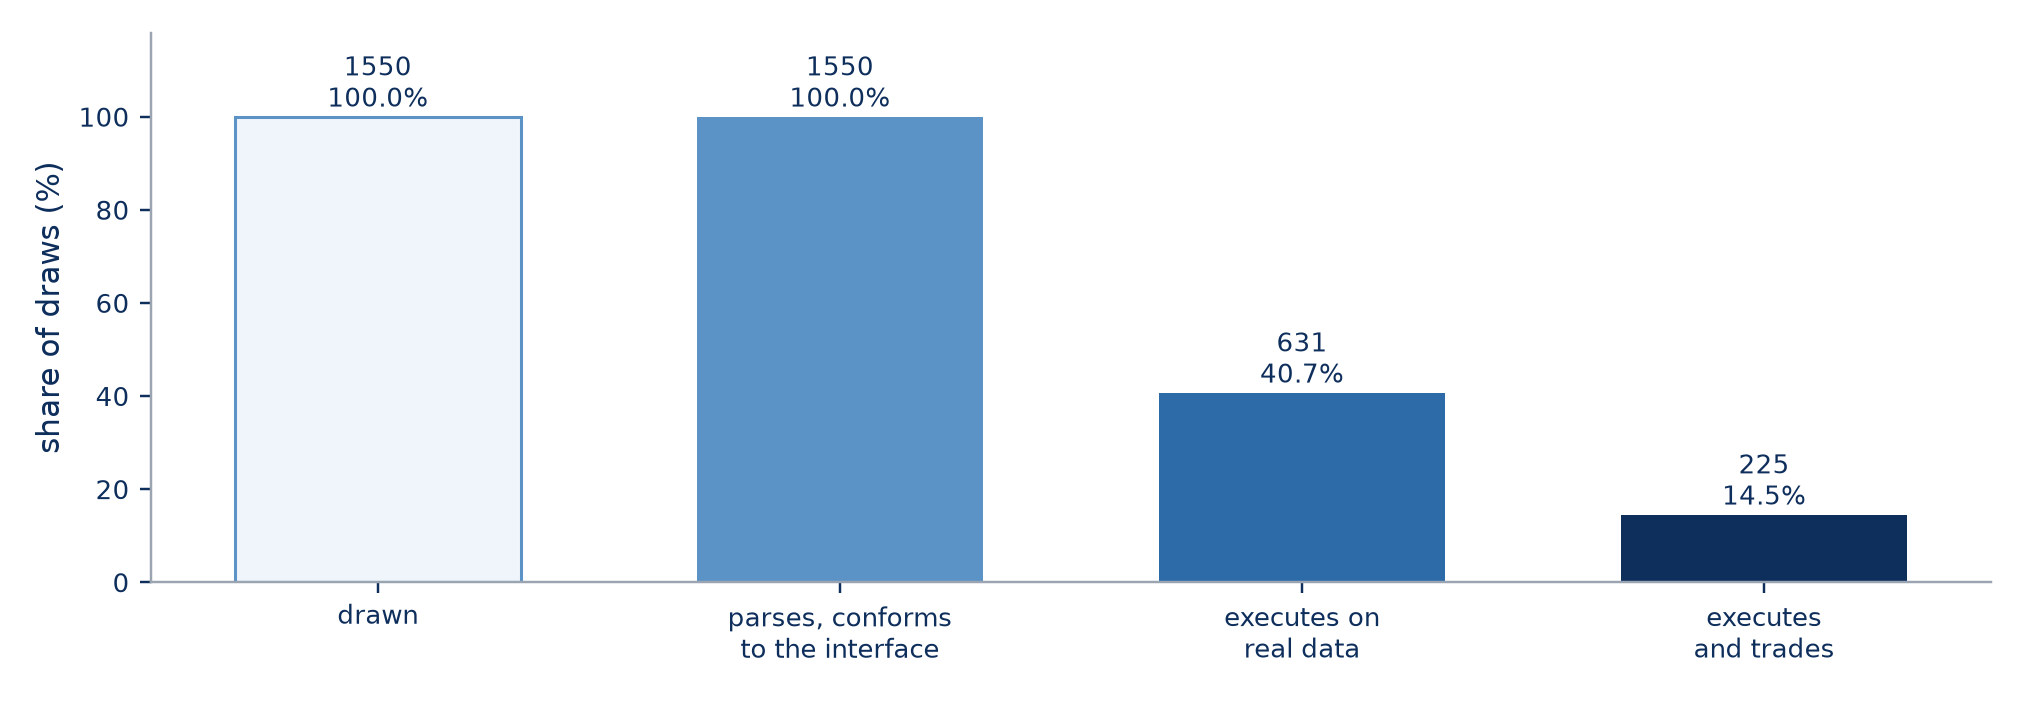
\includegraphics[width=\linewidth]{figures/fig_local_funnel.png}
\caption{The funnel. $n=\aaLocalDraws{}$ draws, one model, one prompt. \textbf{Everything the model
returned was parseable and interface-conforming; almost nothing survived contact with real data.}
Of the candidates that executed, most ran their full course without ever
taking a position --- a failure mode that produces no error and would be invisible to any check
that only asks whether the code ran.}
\label{fig:localfunnel}
\end{figure}


\takeaway{Read the second row. \emph{Every} draw returned syntactically valid Python defining a
conforming strategy with a rationale. The model is entirely reliable at producing code that looks
right. All the attrition happens on contact with data.}

The 894 runtime errors are dominated by a single confusion. \texttt{AttributeError} (327) and
\texttt{ColumnNotFoundError} (247) together account for 64\% of failures, and both trace
overwhelmingly to the model calling pandas methods on polars frames, or treating a wide frame as
though it were long. The prompt states the distinction explicitly and carries a worked example.
The model makes the error anyway, in roughly a fifth of all draws.

\begin{finding}
This relocates the question the project was built to ask. ``What fraction of LLM-generated
strategies fail static leakage screening'' presumes leakage is the binding constraint. On this
corpus it is not: the auditor was never reached for 59\% of the corpus, and for a further 26\% it
had nothing to deflate. \textbf{An auditor tuned to catch cheating is guarding a door most
candidates never reach.}
\end{finding}

\subsection{Leak classes, and one number we do not believe}
\label{sec:leakclasses}

Static analysis needs no execution, so it ran over all 1{,}550 sources: \aaLocalStatic{} rejected
(\aaLocalStaticPct\%), of which 195 carried one class, 26 two, and one three.

\begin{figure}[h]\centering
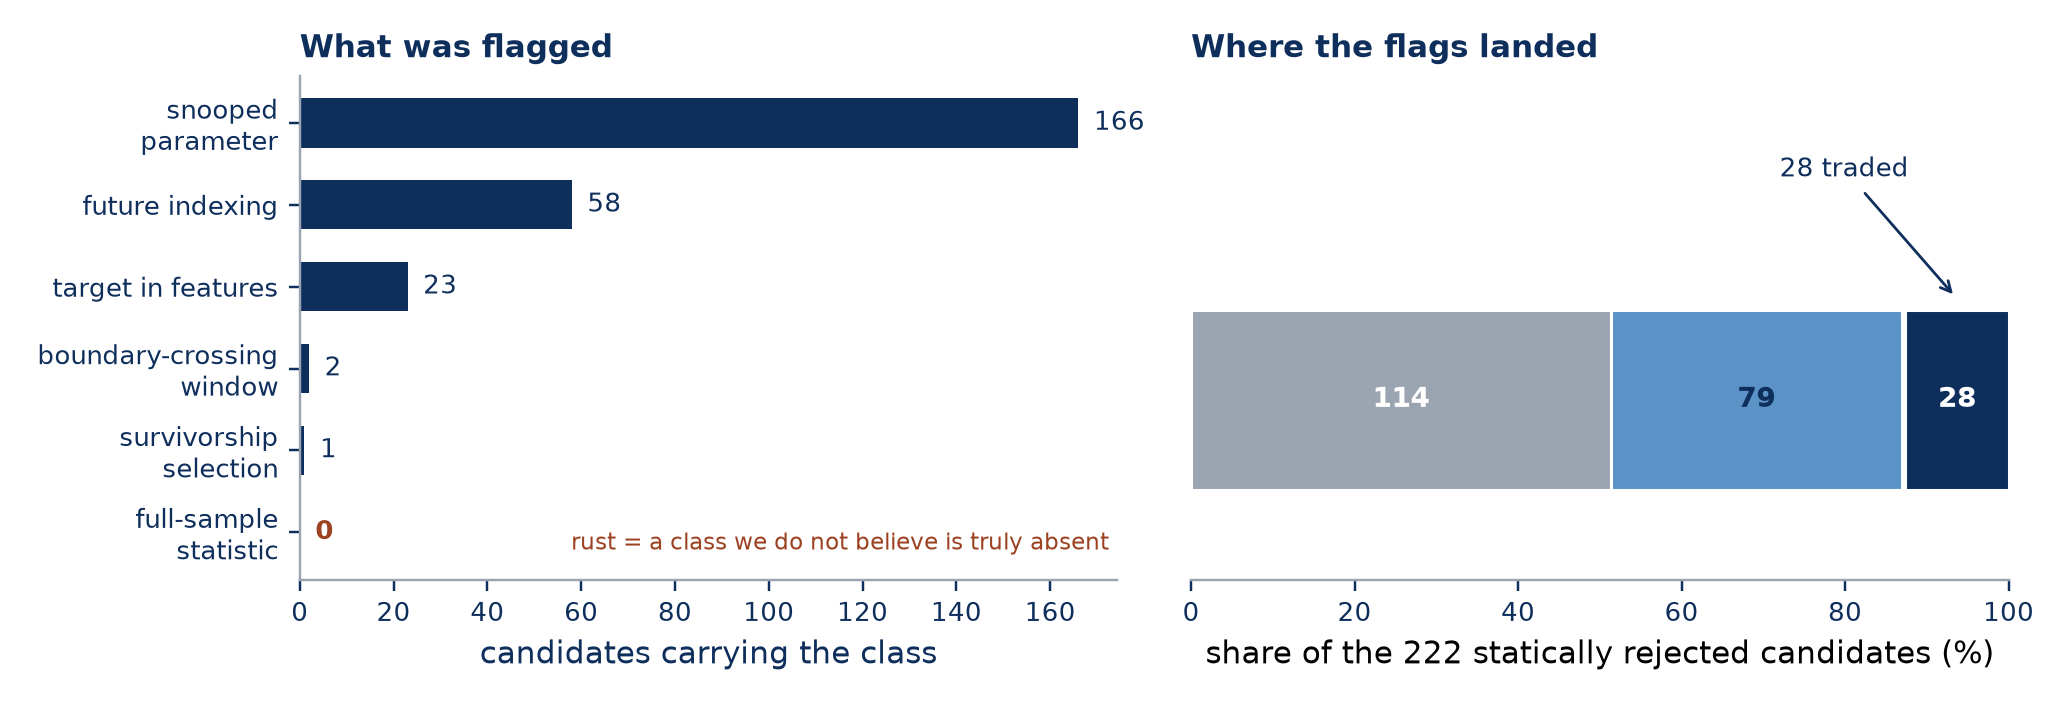
\includegraphics[width=\linewidth]{figures/fig_leak_classes.png}
\caption{\emph{Left:} what the static auditor found across all \aaLocalDraws{} sources, by class.
One class dominates and one is empty, and the empty one is the finding --- see below.
\emph{Right:} what became of the \aaLocalStatic{} candidates it rejected. \textbf{Almost every
flag landed on code that never took a position}, so a leakage-prevalence rate measured over
generated source is not a deployment-risk rate.}
\label{fig:leakclasses}
\end{figure}


\begin{selfreport}[title={We do not believe the zero}]
Full-sample statistics are the most common leak class in hand-written quantitative code, and a
corpus of 1{,}550 candidates containing none of it is not plausible. The cause is almost certainly
ours: to raise the executable rate from near zero, the prompt advises working in plain Python
rather than in long polars expression chains, and \texttt{pl.col("x").mean()} over an unfiltered
frame is precisely where this class arises. The distribution above therefore describes
\textbf{this prompt}, not LLM-generated strategies in general, and the zero should be read as
evidence that the instrument is blind here --- not that the defect is absent.
\end{selfreport}

\paragraph{Most leak flags land on code that never produced a result.} Static analysis is a
statement about source, not about realised profit, and the two are correctly independent: a leak
is a leak whether or not the strategy went on to trade. But \emph{where} the flags land is itself
a measurement.

The right-hand panel of Figure~\ref{fig:leakclasses} shows where they landed.


\noindent \textbf{Only \aaLocalStaticRankable{} leak findings in the entire corpus attach to a
strategy that took a position.} A worked example makes the mechanism concrete. Candidate 053 is
flagged \texttt{future\_indexing} at confidence 1.0 for a \texttt{shift(-1)} whose result is then
filtered onto a past session date --- textbook future indexing, correctly caught. But the block is
unreachable: the guard preceding it requires 21 rows from a view that returns at most 20, so it is
false on every session and the function exits before the leak executes. Had it been reached it
would have raised twice over.

The verdict and the flat return series are compatible, not contradictory. What the pairing shows
is that \textbf{a leakage-prevalence rate measured over generated source is not a deployment-risk
rate}. Reported as ``\aaLocalStaticPct\% of candidates leak'', the static layer sounds like it is
intercepting a substantial hazard. Reported as ``\aaLocalStaticRankable{} of 1{,}550 candidates
leak \emph{and} trade'', the same measurement says the hazard is rare because the population is
inert. Both numbers are true. Only the second is decision-relevant, and we are not aware of prior
work that separates them.

\medskip
The semantic layer labelled 90.1\% of the corpus \texttt{consistent}, rejecting 154 (9.9\%): 119
rationale--implementation mismatches, 21 unacknowledged known anomalies, 14 unfalsifiable
mechanisms. It is not a detector that fires indiscriminately. Whether the 154 are the \emph{right}
ones is not established on this population, since $\kappa$ was measured on a different one.

% =====================================================================================
\section{The frontier-model comparison}
\label{sec:frontier}

\begin{finding}
\tagfrontier\ \ \textbf{Frontier models solved the execution problem. They did not solve the
evidence problem.}
\end{finding}

The obvious objection to \S\ref{sec:local} --- and the first one a referee reaches for --- is that
we measured a small local model, not AI strategy generation. So the identical frozen task
specification was issued to three frontier models, and every candidate was run through the
identical unchanged funnel. \textbf{This is not an appendix.} The generator is part of the
scientific design, because the programme's question is what changes when the AI gets better.

\aaGvRequestsPerArm{} requests per arm, \aaGvTotal{} candidates in total, \aaGvNLarge{} per arm.

\begin{figure}[t]\centering
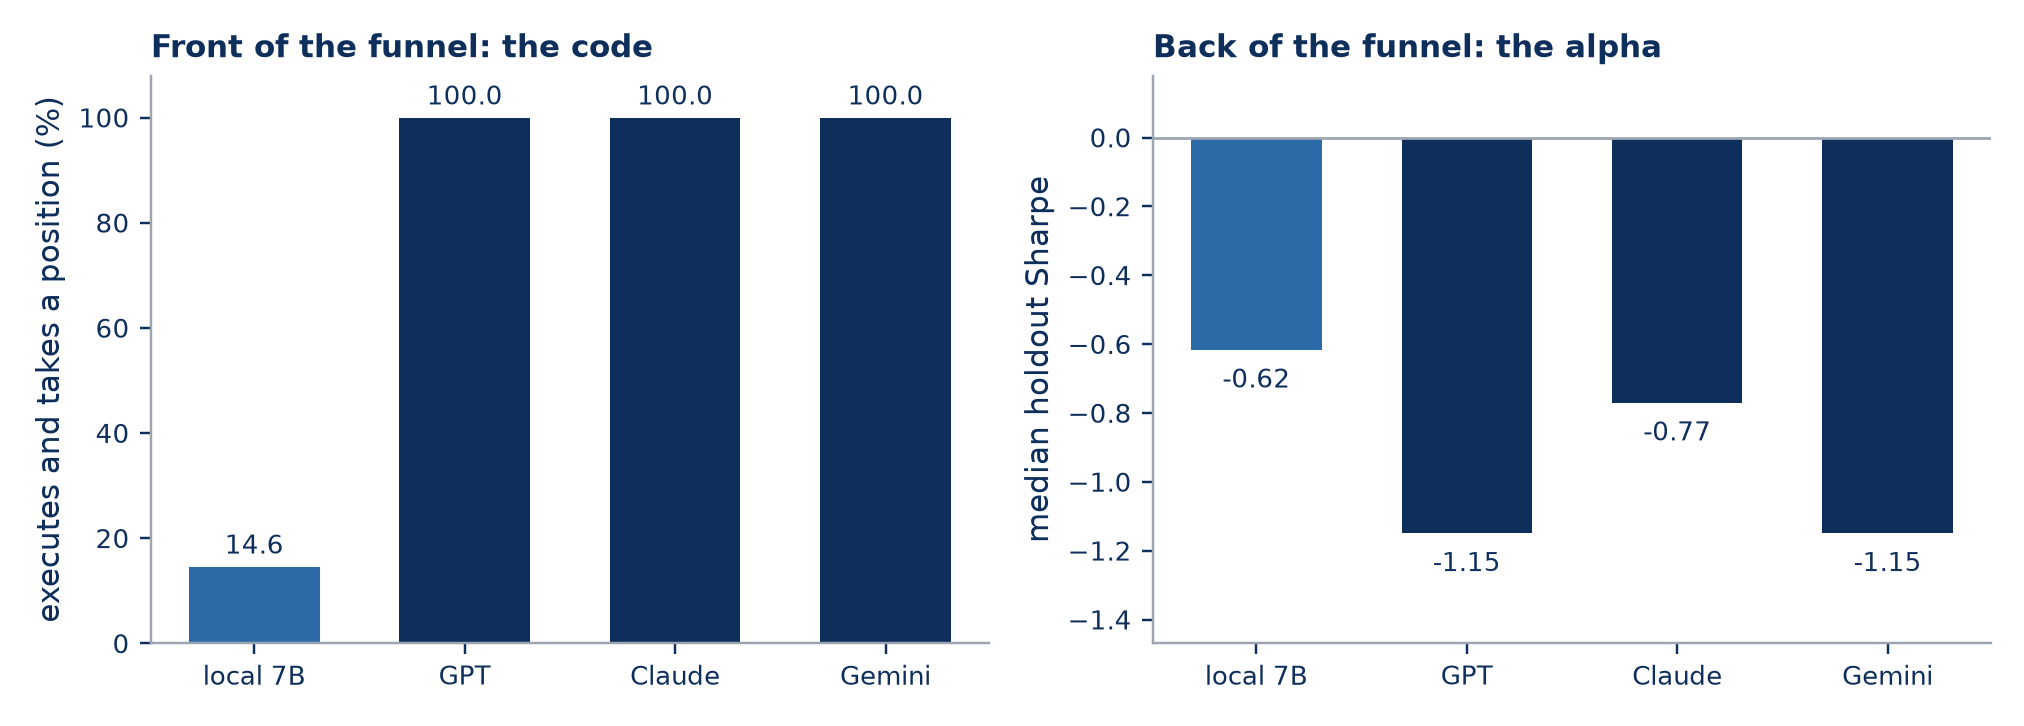
\includegraphics[width=\linewidth]{figures/fig_front_vs_back.png}
\caption{The same generators on one axis, measured at two points in the funnel. Left: the fraction
of draws producing code that runs on real data and takes a position. Right: median Sharpe on the
never-touched holdout year. Sample sizes differ by up to $40\times$ between the reference and the
frontier arms; see the scope box below.}
\label{fig:frontback}
\end{figure}

\takeaway{Capability moves the left panel to its ceiling and does not move the right panel in the
direction that would matter.}

\subsection{The front of the funnel: solved}

\begin{figure}[t]\centering
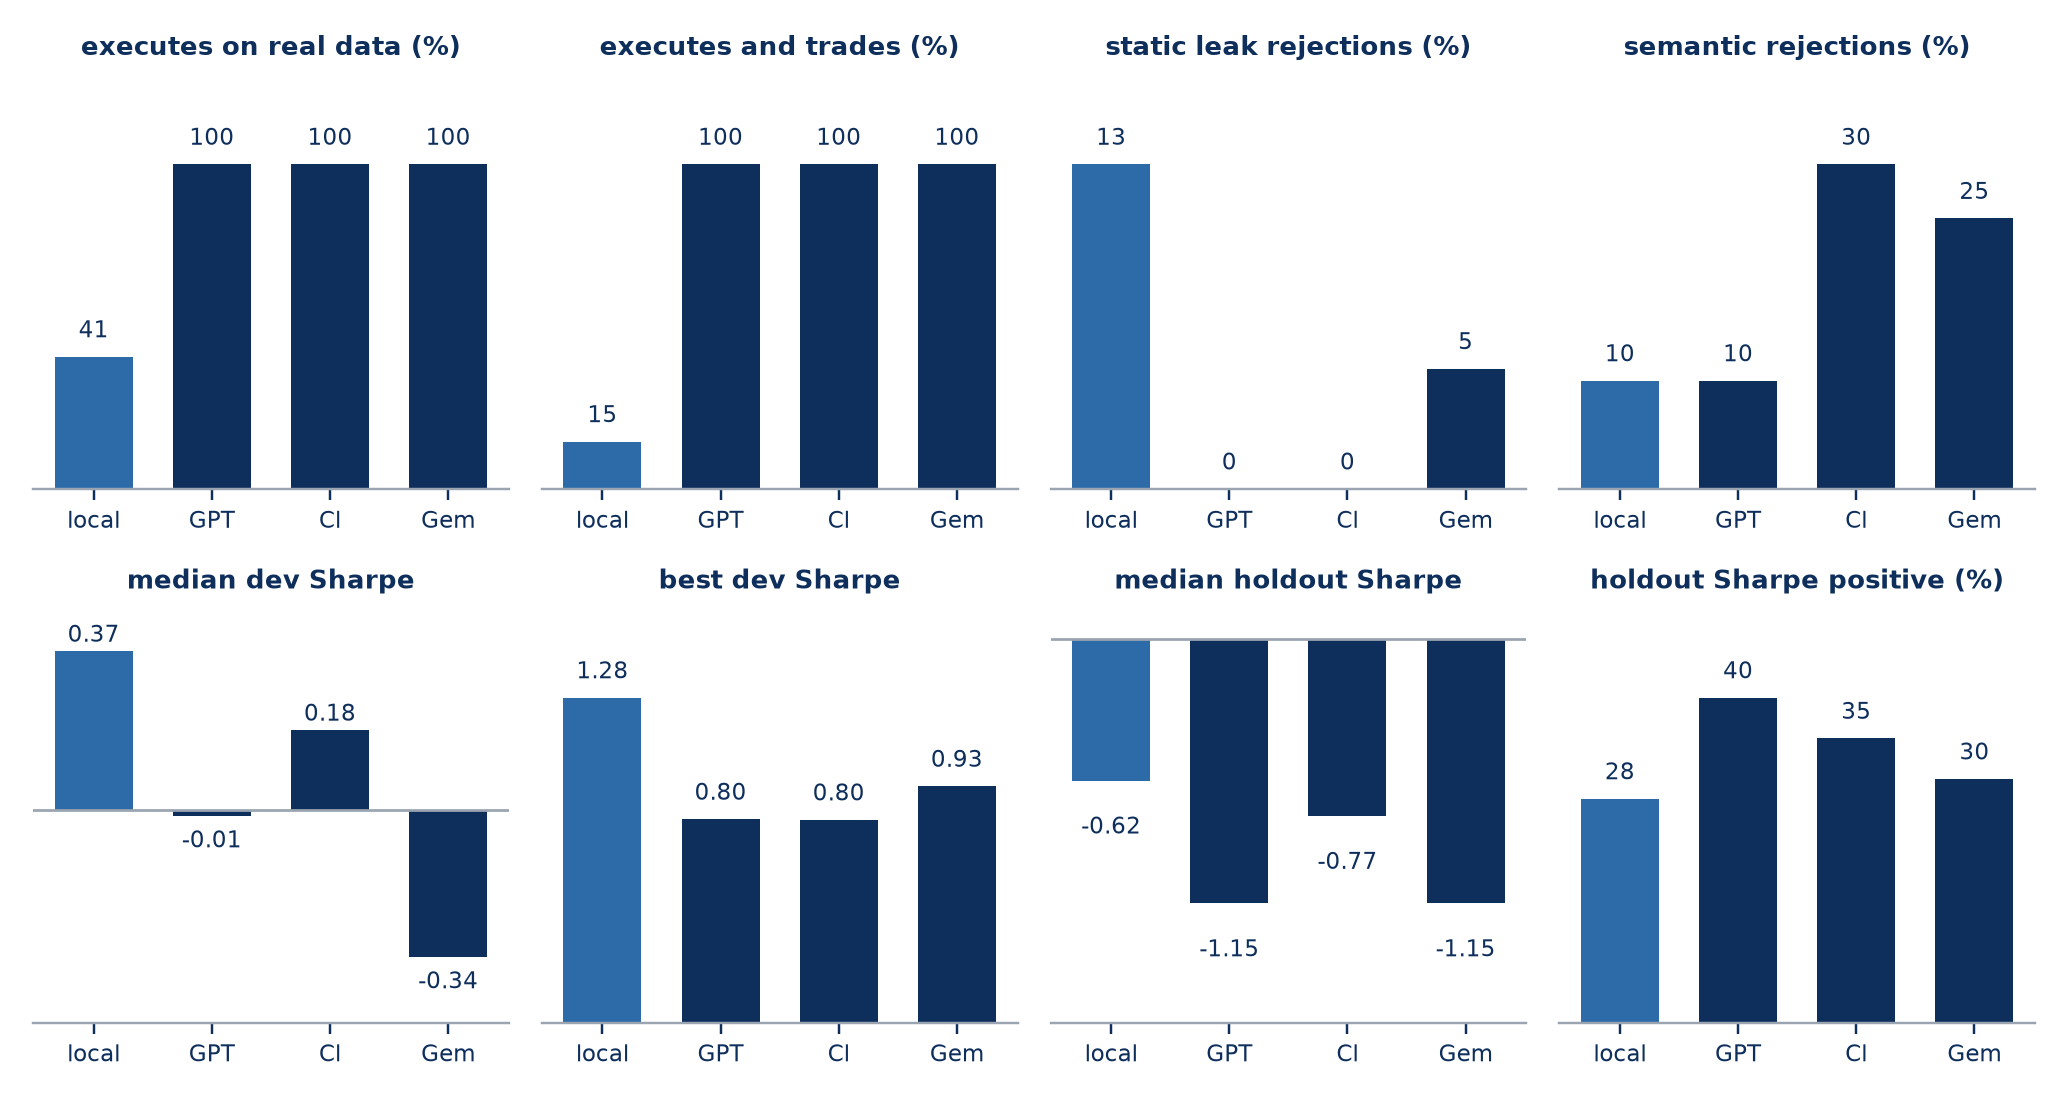
\includegraphics[width=\linewidth]{figures/fig_frontier_axis.png}
\caption{The generator axis: identical prompt, identical funnel, \textbf{not compute-matched} ---
these are rate claims only, never efficiency claims. Each quantity gets its own panel because they
share no unit. \textbf{The top row moves and the bottom row does not.} Draws are \pgmPlainDraws{}
locally and \aaGvGptN{} on each frontier arm. The statistical layer is not plotted because it
rejected \emph{every} strategy on \emph{every} arm --- a flat row of four identical bars, and
\S\ref{sec:factors} is where that gets taken seriously.}
\label{fig:frontier}
\end{figure}


Every frontier arm executed and traded at 100\%. The execution barrier that consumes 85\% of the
local corpus is not a property of machine-written strategies; it is a property of a 7B model, and
it vanishes with capability. Total static leak findings across all \aaGvTotal{} frontier
candidates: \aaGvStaticTotal{}. Frontier models do not write the cheats our static layer was built
to detect --- but note that the local corpus barely did either
(\aaLocalStaticRankable{} of 1{,}550 that both leaked and traded), so this is a small effect
measured on a small sample, not a demonstration that capability eliminates leakage.

\subsection{The back of the funnel: unmoved}

\begin{finding}
\tagfrontier\ \ \textbf{Zero of \aaGvTotal{} frontier candidates cleared the significance bar} at
their own honest trial counts, on development or on holdout. The local corpus cleared 0 of 631.
Capability changed the numerator of the funnel by a factor of seven and left this at zero.
\end{finding}

Every frontier arm's median holdout Sharpe is \emph{worse} than the local reference's, and every
arm's mean is negative on both windows. The best single holdout Sharpe in any frontier arm is
\aaGvClaudeHoldBest{} --- positive, but nowhere near clearing deflation at that arm's own trial
count, and selected as the maximum of twenty.

\begin{scopebox}
\textbf{The supportable claim is that frontier models did not \emph{improve} out-of-sample
performance --- not that they produced none.} Three things block the stronger claim.
\begin{itemize}
\item Median holdout Sharpe is worse for all three arms, but the \emph{fraction} with a positive
  holdout Sharpe is better: 40\%, 35\% and 30\% against the local arm's \pgmPlainHoldPos\%.
  Those two facts point in opposite directions and we report both.
\item The populations are differently selected. The local arm's \pgmPlainHoldPos\% is measured on
  the \pgmLocalTrade\% of draws that survived execution; the frontier arms' on 100\% of draws.
  The local survivors passed a filter the frontier candidates never faced.
\item \textbf{The generator axis is not compute-matched.} \aaGvNLarge{} frontier draws against
  \pgmPlainDraws{} local draws, at unequal and unmeasured token cost. Under Rule 11 of this
  programme's charter no generator-axis comparison may be reported as an efficiency win, and none
  is.
\end{itemize}
\end{scopebox}

\subsection{The matched-size control, and why small samples flatter}

Comparing a 20-draw arm against a 1{,}550-draw corpus is not a fair deflation comparison, because
deflation punishes trials: a 20-trial arm faces a much lower bar than a 1{,}550-trial one. So we
drew \aaGvSubsamples{} random subsamples of the local corpus at each frontier arm's size and
deflated each subsample at its own trial count, recomputing trial dispersion \emph{within} the
subsample --- because that is the only information a 20-draw arm actually has.

\begin{center}\small
\begin{tabular}{lrr}
\toprule
\thead{Subsamples of the local corpus clearing DSR $\ge \aaGvBar{}$} & \thead{at $n=\aaGvNSmall{}$}
  & \thead{at $n=\aaGvNLarge{}$} \\
\midrule
Development window & \aaGvMatchedDevSmall{}/\aaGvSubsamples{} &
  \aaGvMatchedDevLarge{}/\aaGvSubsamples{} \\
\textbf{Holdout} & \textbf{\aaGvMatchedHoldoutSmall{}/\aaGvSubsamples{}} &
  \textbf{\aaGvMatchedHoldoutLarge{}/\aaGvSubsamples{}} \\
\bottomrule
\end{tabular}
\end{center}

\takeaway{On development, a five-draw slice of the \emph{local} corpus clears the bar 4.1\% of the
time --- purely because five trials are cheap to deflate. No frontier arm cleared it at twenty. On
the holdout, nothing clears at any size: \aaGvMatchedHoldoutSmall{} of \aaGvSubsamples{} local
subsamples, and \aaGvClearedHoldout{} of \aaGvTotal{} frontier candidates. This is the control
that shows the frontier arms' failure is not a small-sample artefact.}

\subsection{Two vendors wrote the same strategy, and it was the median}

\begin{finding}
\tagfrontier\ \tagexpl\ \ Three GPT candidates and two Gemini candidates produce holdout return
series \textbf{identical to within $8.7\times10^{-19}$ across all 245 sessions} --- the same
turnover, the same volatility, the same return. Two different vendors, given the same prompt,
converged on behaviourally identical code. \textbf{That cluster sits exactly on the median of both
arms}, which is why GPT and Gemini report the same median holdout Sharpe to sixteen decimal
places (\pgmGPTHoldMed{} and \pgmGeminiHoldMed).
\end{finding}

This was found while checking whether the identical medians were a bug. They are not; they are a
measurement. Duplicate clustering is not a local-model pathology --- it recurs at the frontier,
across vendors. It also means a per-arm mean or median can be a statement about one duplicated
idea rather than about twenty independent ones, and any comparison across these arms inherits that.

\begin{scopebox}
This is an \textbf{exploratory} finding: it was not pre-registered, it was discovered while
verifying another number, and it rests on five candidates. It is reported because it materially
affects how the medians in Figure~\ref{fig:frontier} should be read, not because five candidates
establish a general property of frontier models.
\end{scopebox}

% =====================================================================================
\section{Advanced generation methods, at equal compute}
\label{sec:methods}

\begin{finding}
\tagmethod\ \tagprereg\ \ \textbf{Of \pgmScaffoldArms{} scaffolded generation methods,
\pgmScaffoldWins{} beat plain prompting once plain prompting was given the same token budget.}
\end{finding}

If capability does not help, perhaps method does. The same local model, the same frozen task
specification, and \pgmParadigmArms{} generation methods: plain prompting, chain-of-thought
\citep{wei2022}, planning, reflection \citep{shinn2023}, graph-of-thoughts \citep{besta2024}, and
Monte Carlo tree search over candidate programs \citep{yao2023}. \pgmParadigmDraws{} draws in
total.

\subsection{Why the naive comparison is worthless}

A five-agent committee that spends five times the tokens of a single prompt and produces better
output has demonstrated nothing. Of course it does --- it thought five times as hard. The honest
control is not plain prompting at its natural budget; it is \textbf{plain prompting run $k$ times
at the same total token budget, allowed to keep its best}. We compute $k$ from measured tokens per
accepted strategy, and we count barren blocks in the denominator so that a method is not rewarded
for the attempts it wasted.

\begin{figure}[t]\centering
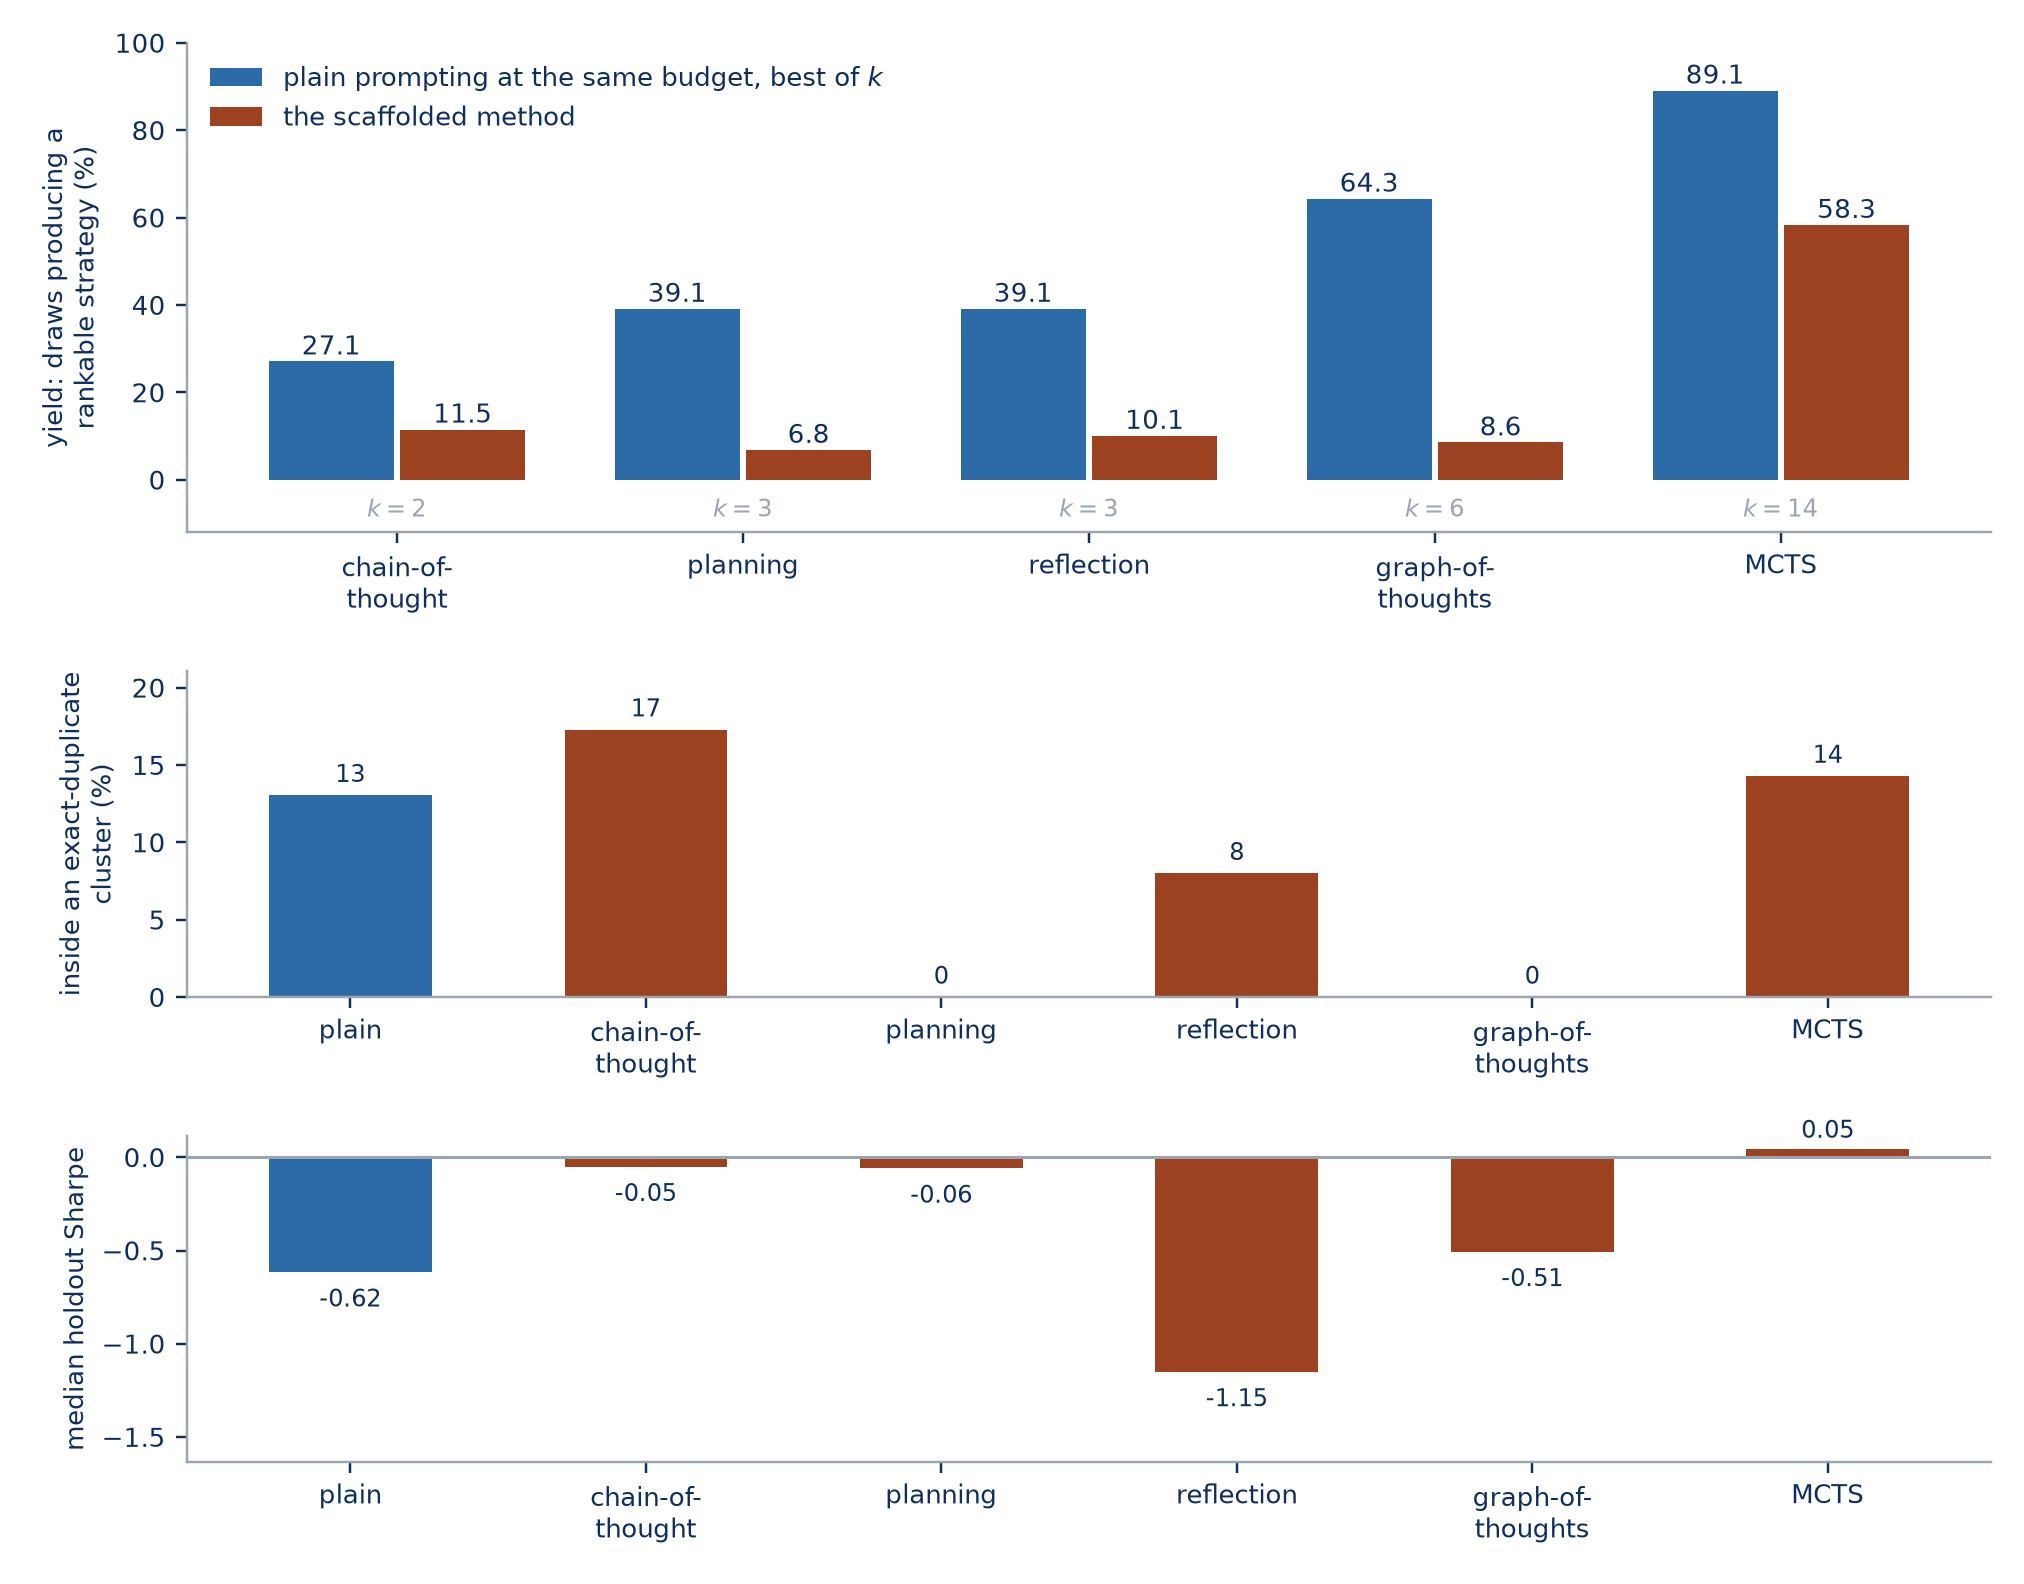
\includegraphics[width=\linewidth]{figures/fig_compute_matched.png}
\caption{The methodology axis, all on the same local model. \emph{Top:} each scaffolded method
against plain prompting at the same measured token budget, where $k$ is the number of
plain-prompting attempts the scaffolded method's token spend buys. \emph{Middle and bottom:} the
two panels a yield comparison alone would have missed --- a method that collapses onto one idea and
repeats it scores well on average and is worth nothing, and a method that raises yield without
raising out-of-sample performance has produced code rather than research.}
\label{fig:matched}
\end{figure}

\takeaway{Every scaffolded method loses to its own control. The gap widens with the amount of
scaffolding: graph-of-thoughts spends $k=\pgmGraphK{}$ plain prompts' worth of tokens per
strategy, and tree search spends $k=\pgmMctsK{}$.}


\begin{figure}[t]\centering
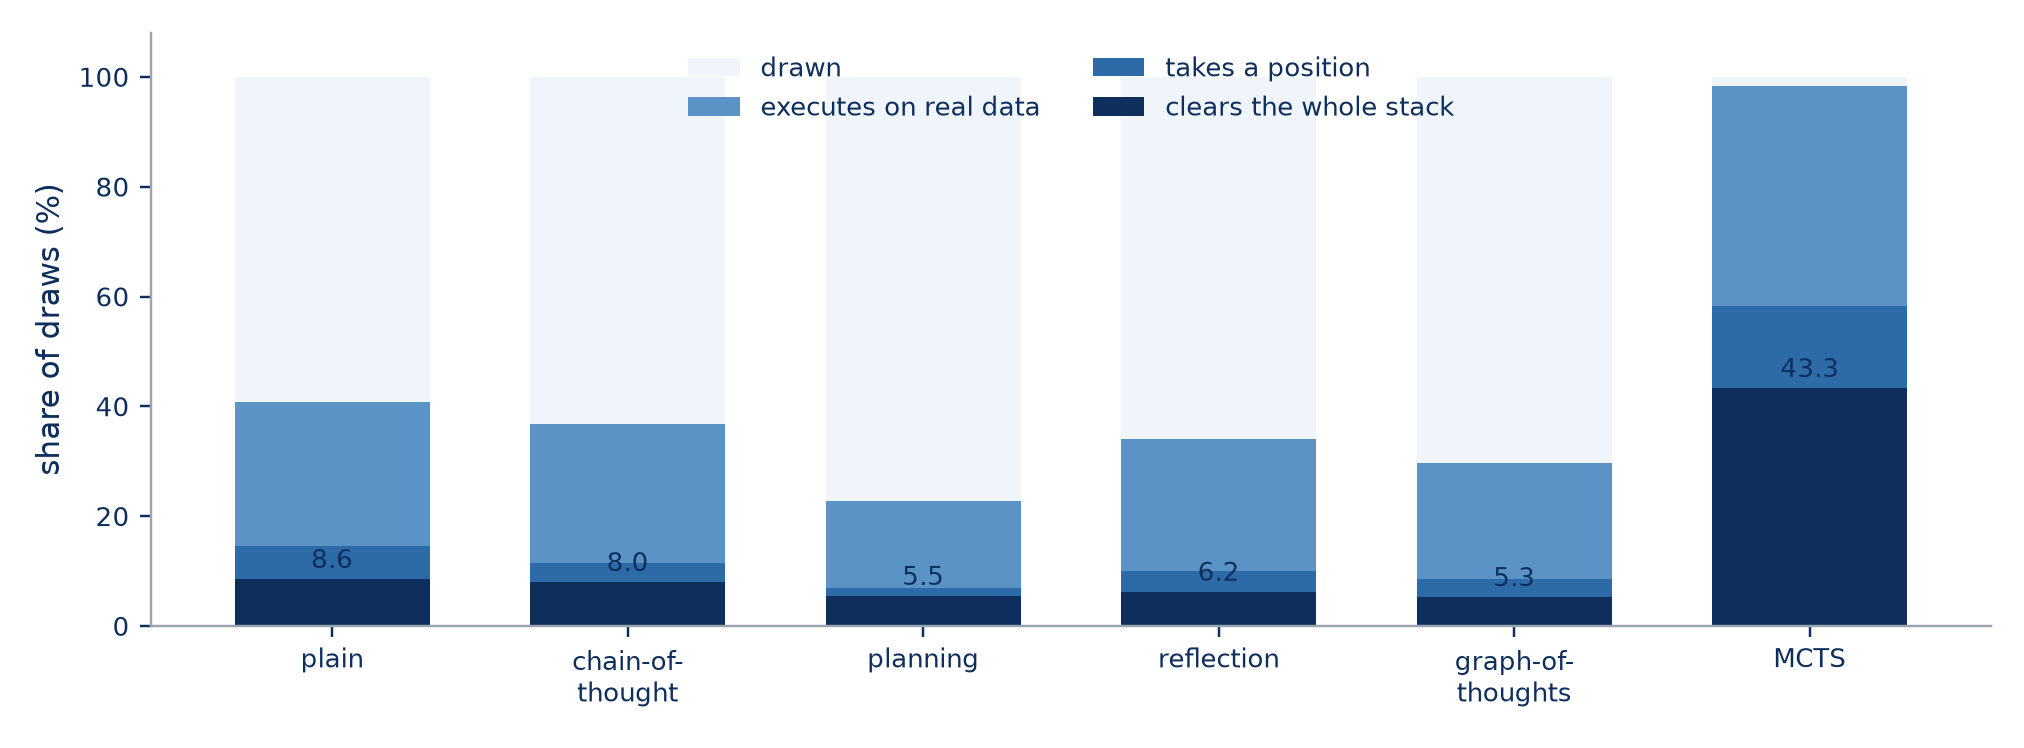
\includegraphics[width=\linewidth]{figures/fig_funnel.png}
\caption{Where each method's corpus dies, as a share of its own draws. The dark bar is the share
clearing the entire evaluation stack.}
\label{fig:funnel}
\end{figure}

\subsection{The one arm that looks like a win, and why we do not report it as one}

Tree search reaches \pgmMctsTrade\% yield and \pgmMctsSurv\% full-stack survival against plain
prompting's \pgmPlainTrade\% and \pgmPlainSurv\% --- by far the highest in the programme. It is
also the arm whose compute-matched control is highest of all, at \pgmMctsCtrlYield\% against its
own \pgmMctsTreatYield\%.

\begin{scopebox}
\textbf{Tree search is treated as an anomaly to investigate, not an effect to report}, on the
principal investigator's ruling and for three reasons stated before its downstream numbers were
examined. Its sample is the smallest in the programme (\pgmMctsDraws{} draws). Its $k$ is the
largest (\pgmMctsK{}), so its control is correspondingly generous. And a jump of this size in this
domain is, on the programme's own standing rule, more likely to be a defect than a discovery. We
did not delete the arm --- deleting an inconvenient arm is worse than reporting a confusing one
--- and we do not claim it as a win.
\end{scopebox}

\subsection{Does scaffolding trade diversity for quality?}

The hypothesis stated in advance was that heavier scaffolding induces mode collapse: quality rises
while diversity falls. The measurement is redundancy --- the share of a method's tradeable output
sitting inside a cluster of behaviourally identical return series, detected by union-find over
realised returns.

Redundancy does not rise with scaffolding: chain-of-thought is highest at \pgmCotRedund\%,
and planning and graph-of-thoughts report \pgmPlanRedund\% and \pgmGraphRedund\%. But those two
zeros are \textbf{not evidence of diversity}, and this is a case where reporting the number
without its power would mislead. At the reference duplicate rate observed in the two large arms, a
sample of planning's size would return zero duplicates by chance \pgmPlanPZero\% of the time, and
one of graph-of-thoughts' size \pgmGraphPZero\% of the time. \textbf{Those zeros are consistent
with the same duplication rate as everything else.} Only the two large arms have the power to say
anything: there, zero duplicates would occur \pgmPlainPZero\% and \pgmCotPZero\% of the time, and
duplicates were observed.

\takeaway{We cannot confirm or reject the mode-collapse hypothesis on the small arms. Saying so is
the result; quoting the zeros as diversity would not be.}

Cross-arm duplication is the sharper measurement, since it does not depend on within-arm sample
size: \pgmPlainXArm\% of plain prompting's tradeable output and \pgmCotXArm\% of
chain-of-thought's is behaviourally identical to something another arm produced. Different
methods, same strategies.

% =====================================================================================
\section{What survives costs, multiple testing and the holdout}
\label{sec:survives}

\subsection{Costs are a selection mechanism}

\begin{table}[t]\centering\small
\caption{Gross to net over the development window, local corpus. $n=\aaLocalRankable{}$ traded
candidates. Gross and net come from a \emph{single run} --- the engine records the pre-cost series
alongside the post-cost one --- so the drag is a measured quantity on one path, not a difference
between two runs.}
\label{tab:grossnet}
\begin{tabular}{lrr}
\toprule
\thead{Quantity} & \thead{Value} & \thead{Sample} \\
\midrule
Best Sharpe, gross & 1.3049 & \aaLocalRankable{} \\
Best Sharpe, net & \textbf{1.2807} & \aaLocalRankable{} \\
Mean Sharpe reduction & \aaLocalCostDrop{} & \aaLocalRankable{} \\
\textbf{Median} Sharpe reduction & \textbf{0.1943} & \aaLocalRankable{} \\
Mean turnover, annualised & 82.2$\times$ & \aaLocalRankable{} \\
Median turnover, annualised & 17.6$\times$ & \aaLocalRankable{} \\
Mean cost drag, annualised & 58.13\% & \aaLocalRankable{} \\
Median cost drag, annualised & 4.39\% & \aaLocalRankable{} \\
\textbf{Sharpe sign reversed, $+\!\rightarrow-$} &
  \textbf{\aaLocalFlips{} (\aaLocalFlipsPct\%)} & \aaLocalRankable{} \\
Sharpe sign reversed, $-\!\rightarrow+$ & \textbf{0} & \aaLocalRankable{} \\
Ruined outright (equity reached zero) & 11 & 631 \\
\bottomrule
\end{tabular}
\end{table}

Mean and median diverge by a factor of thirteen on cost drag. The mean is dragged by a tail
churning above $80\times$ annual turnover; the median strategy loses 0.19 of Sharpe and 4.4\% a
year. Both are reported because quoting either alone misleads.

The best gross strategy is also the best net strategy --- because it barely trades, at
$2.8\times$ annual turnover and 0.4\% annual cost. \textbf{Cost survival selects for low turnover,
not for skill}, the same conclusion \citet{novymarx2016} reach for US anomalies, arrived at here
through a very different door.

\paragraph{Standard factors are not spared.} Eleven textbook factors through the same pipeline as
a positive control: drag rises monotonically with turnover in ten of eleven rows, and two factors
flip from profitable to unprofitable. Momentum \citep{jegadeesh1993} survives at a net Sharpe of
0.9656 --- but equal-weighting the same universe returns 0.9615. \textbf{Net of Indian costs, the
momentum premium on this universe is inside the noise.}

\paragraph{The eleventh row, and why the assumed book size decides the verdict.} The one factor
breaking monotonicity is inverse-volatility weighting: the \emph{lowest} turnover of any active
strategy (0.011 per session) and the second \emph{highest} cost (10.18 bps per session). It holds
a hundred names and nudges each daily, and the depository charge is levied per scrip regardless of
size.

\begin{table}[h]\centering\small
\caption{Depository-charge contribution by book size, obtained by differencing against a no-DP
ablation rather than recomputed from the rate.}
\label{tab:dp}
\begin{tabular}{llrrrr}
\toprule
\thead{Strategy} & \thead{Book} & \thead{Total bps/day} & \thead{DP bps/day} &
\thead{DP share} & \thead{Sharpe} \\
\midrule
inverse\_volatility & \rupee 10 L  & 10.183 & 9.963 & 97.8\% & $-1.3792$ \\
inverse\_volatility & \rupee 1 Cr  & 0.866  & 0.597 & 69.0\% & $+0.6359$ \\
inverse\_volatility & \rupee 10 Cr & 0.590  & 0.059 & 10.0\% & $+0.6922$ \\
\midrule
momentum\_skip\_month & \rupee 10 L  & 1.685 & 0.066 & 3.9\% & 0.9656 \\
momentum\_skip\_month & \rupee 10 Cr & 3.944 & 0.001 & 0.0\% & 0.7506 \\
\bottomrule
\end{tabular}
\end{table}

\takeaway{The depository contribution falls $169\times$ across a $100\times$ book sweep, close to
the inverse proportionality the model predicts, and \textbf{the strategy's verdict reverses with
assumed capital}: $-1.38$ at \rupee 10 lakh, $+0.69$ at \rupee 10 crore. Momentum runs the
opposite way. Small books are killed by flat fees, large books by market impact, and the two
regimes cross over.}

We report the corpus at \rupee 10 lakh, which was the pre-existing default, and we did not change
it after observing that it flips a sign.

\subsection{Nothing clears deflation, on any arm}

At an honest trial count of $N=1{,}887$, \textbf{zero of 631 executed local candidates attain a
deflated Sharpe probability above \aaGvBar{}}; the corpus maximum is $4.4\times10^{-8}$. Zero of
\aaGvTotal{} frontier candidates clear it at their own trial counts. The best frontier deflated
probability in any arm is $4.5\times10^{-39}$.

A layer that rejects everything is either correct about a worthless population or non-informative
under this evaluation regime, and the corpus alone cannot distinguish those. \S\ref{sec:factors}
puts the question to a population where the answer is known in advance, and settles it.

% =====================================================================================
\section{The standard-factor control, and what it does to our own auditor}
\label{sec:factors}

\begin{finding}
\tagexpl\ \ \textbf{The statistical layer rejects momentum.} Eleven published factor strategies,
deflated at their own family trial count, produce \textbf{\sfCleared{} clearing the
\sfBar{} bar} --- the same verdict the layer returns on every machine-written corpus. Its maximum
is \sfMaxDsr{}. \textbf{The auditor's 100\% rejection rate carries no information about who wrote
the strategies.}
\end{finding}

Everything in \S\ref{sec:local}--\S\ref{sec:methods} compares machine-written corpora against one
another. That cannot tell us whether a verdict is about machine authorship or about the market, so
the pipeline also carries \sfN{} standard factor strategies --- momentum, low volatility,
short-term and long-term reversal, relative strength, an equal-weight market reference, and two
deliberate controls including a random walk. They were hand-written as Phase 1.2 fixtures, the set
was frozen before any of them was run, and they were never drawn from any search of ours.

\begin{selfreport}[title={They had never been shown to the statistical layer at all}]
This is a gap we found late and report rather than quietly close. The factors were run through the
static layer (\sfStatic{} rejected of \sfN{}) and through the cost model, and their determinism and
knife-edge behaviour were measured for paper 2 --- but the positive-control artefact carries a
static verdict and nothing else. \textbf{The one population that would make the statistical layer's
rejection rate interpretable had never been put to it.} The deflation below was run on 2026-08-08,
appears in no pre-registration, and is \textbf{exploratory throughout}.
\end{selfreport}

\subsection{Costs are a filter here too}

\begin{figure}[t]\centering
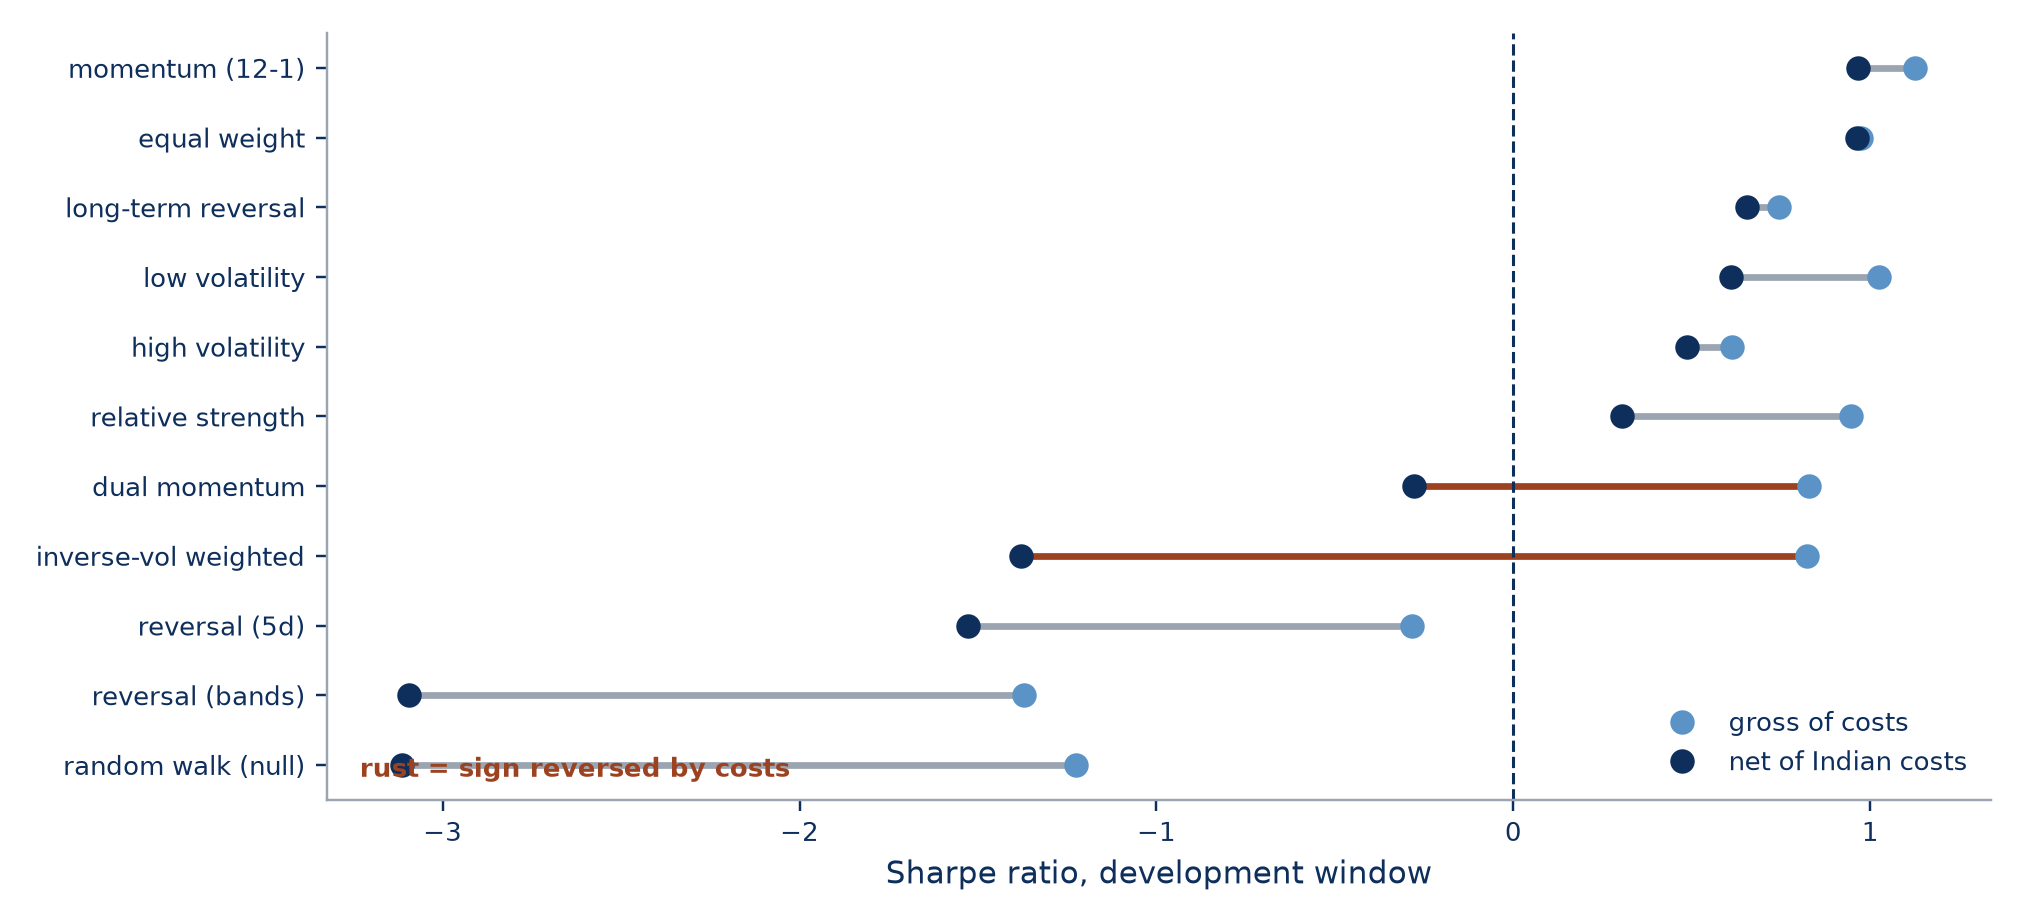
\includegraphics[width=\linewidth]{figures/fig_factor_costs.png}
\caption{Eleven standard factors, gross against net of the Indian statutory schedule. Each row is
one factor; the bar length is what costs take. Rust marks a factor whose Sharpe changes sign.}
\label{fig:factorcosts}
\end{figure}

\takeaway{\sfFlipped{} of \sfN{} factors reverse sign under costs, against
\aaLocalFlipsPct\% of the machine corpus. The median factor gives up \sfMedLost{} of Sharpe. Cost
survival is not a machine-authorship problem; it is a turnover problem, and it applies to
published anomalies exactly as it applies to generated ones.}

Momentum \citep{jegadeesh1993} survives at a net Sharpe of \sfBestNet{} --- but equal-weighting
the same universe returns 0.9615. \textbf{Net of Indian costs, the momentum premium on this
universe is inside the noise.}

\subsection{Deflation rejects all of them}

\begin{figure}[t]\centering
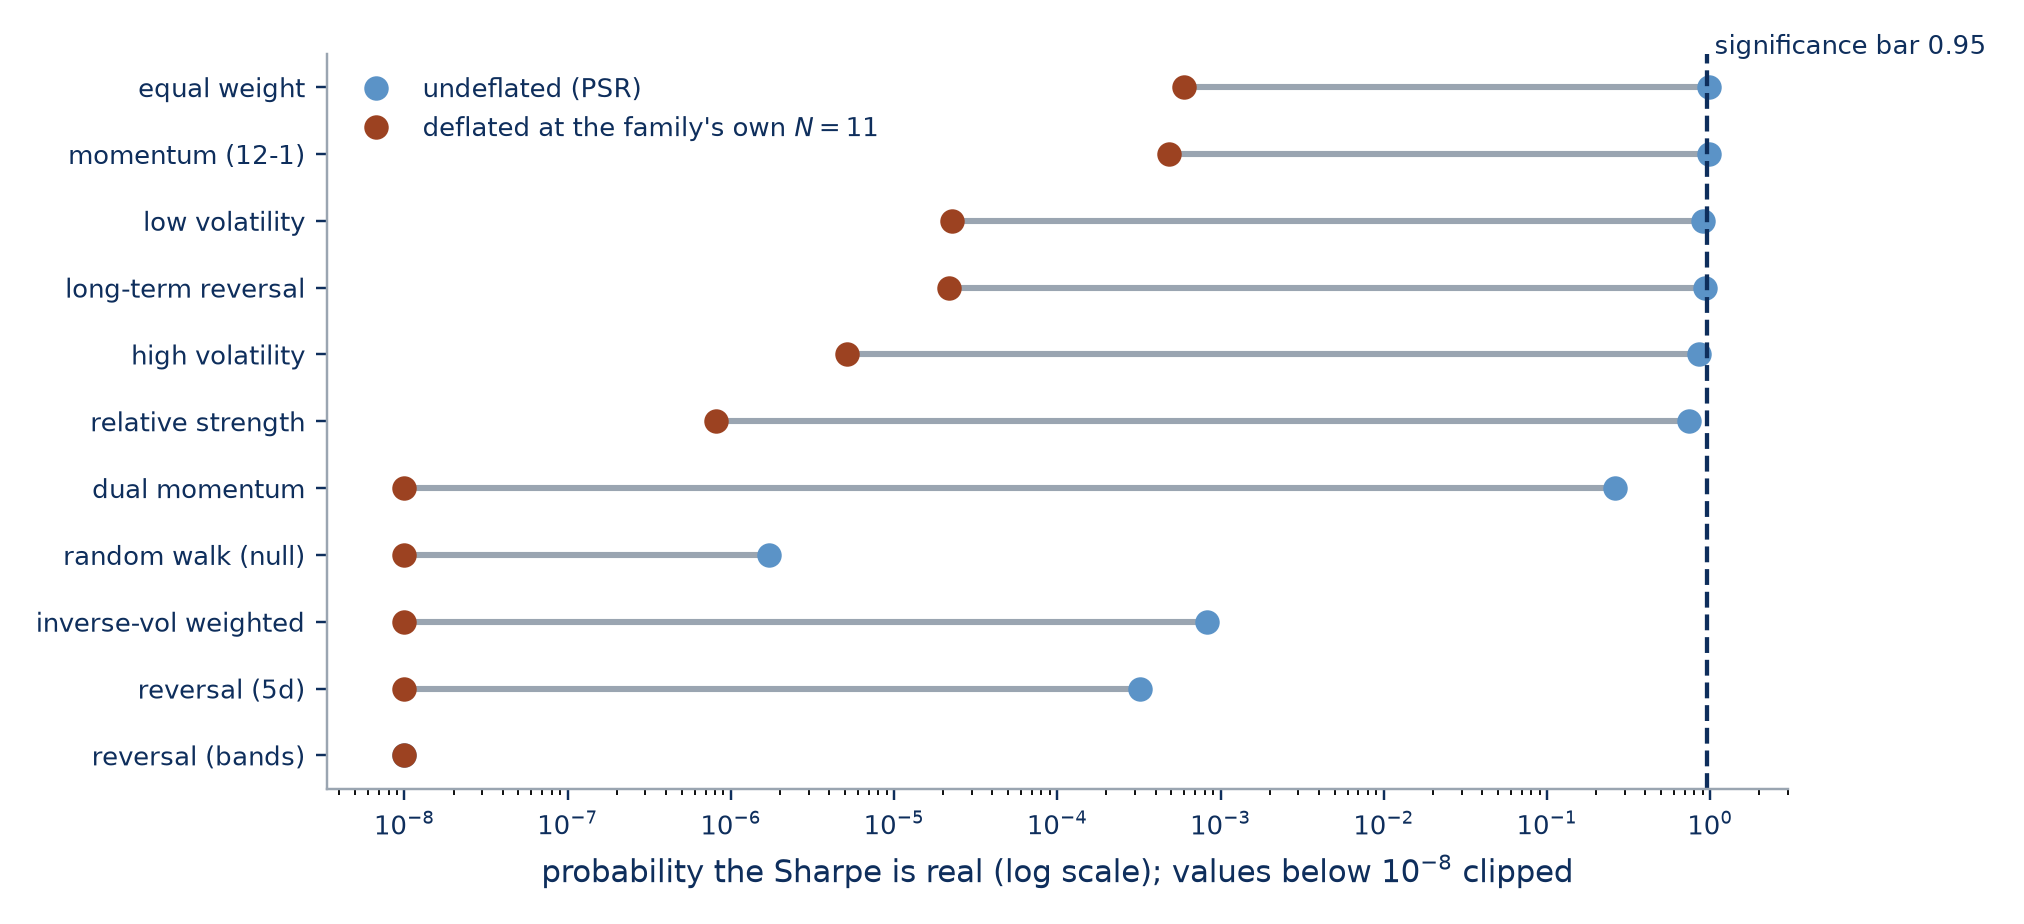
\includegraphics[width=\linewidth]{figures/fig_factor_deflation.png}
\caption{Each factor's significance before and after deflation, at the family's own $N=\sfTrials{}$.
Log scale: the deflated values span twenty orders of magnitude. A factor that cleared the bar would
have its rust dot to the right of the dashed line. None does.}
\label{fig:factordeflation}
\end{figure}

Undeflated, the best factors look conclusive --- momentum's probabilistic Sharpe ratio against zero
is 0.981. Deflated at $N=\sfTrials{}$, it is \textbf{0.00048}. The trial count is barely doing any
work at eleven trials; what sets the bar is the \emph{dispersion} of the comparison family, which
came out at an annualised trial-Sharpe standard deviation of \sfTrialSd{}.

\begin{finding}
The arithmetic, stated so a reader can check it: at $N=\sfTrials{}$ with the measured dispersion,
the luck threshold is \textbf{2.51 annualised}. Momentum's \sfBestNet{} falls \textbf{1.54 short}.
\textbf{To clear \sfBar{} on this window a strategy needs an annualised Sharpe of 3.36} --- against
a best observed of \sfBestNet{}, and against a charter that treats any Sharpe above 1.5 before
costs as an automatic halt-and-investigate condition. \textbf{The auditor's pass bar sits at more
than twice the level at which our own rules require us to presume the result is a bug.}
\end{finding}

\subsection{The mechanism: dispersion, not trial count}

\begin{selfreport}[title={A post-hoc diagnostic, labelled as such because its shape is exactly
  what this lab exists to catch}]
The following was computed \emph{after} seeing the primary result. It is published because it
identifies the mechanism, and it is not a result. Removing strategies from a comparison set until
the number improves is the pathology this programme was built to detect; that we did it knowingly,
to diagnose rather than to flatter, does not exempt it from being labelled.

\begin{center}
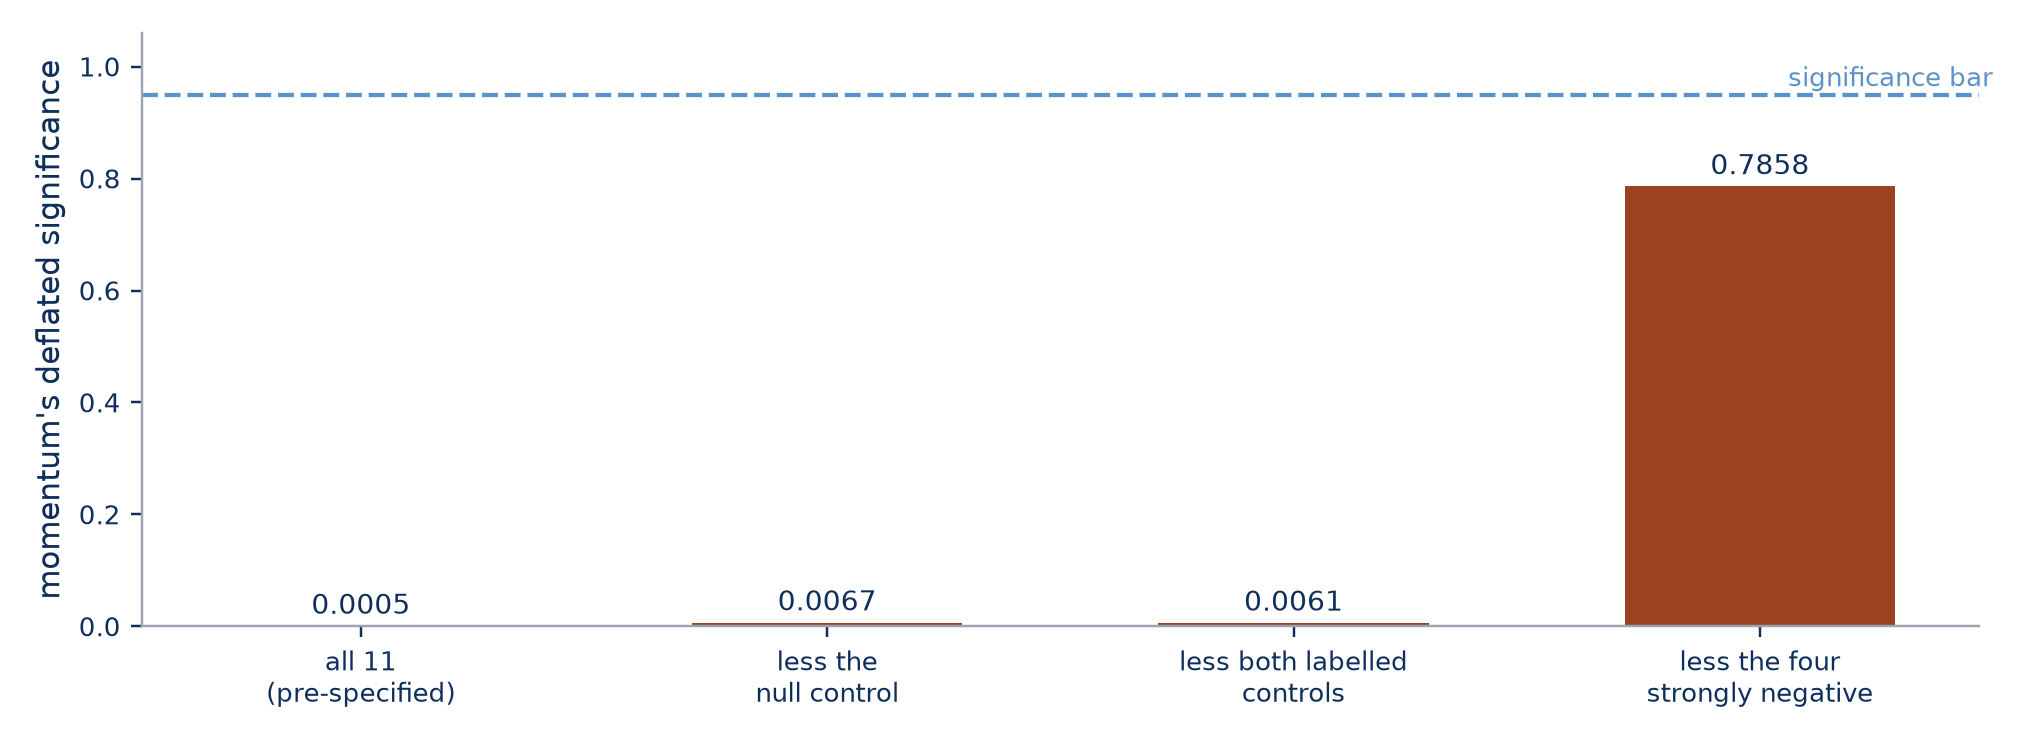
\includegraphics[width=0.92\linewidth]{figures/fig_dispersion_mechanism.png}
\end{center}

\textbf{Same strategy, same Sharpe, same trial count, and a verdict that moves by three orders of
magnitude} --- 0.0005 to 0.786 --- depending only on which other strategies stand beside it. The
Deflated Sharpe Ratio's verdict is dominated by an input the researcher chooses.

The primary figure remains the pre-specified set of all \sfN{}. We do not adopt any of the reduced
sets, and no number anywhere else in this paper uses one.
\end{selfreport}

\subsection{Is the layer broken?}

No, and we checked rather than asserted. The module's 72 tests pass; its expected-maximum-Sharpe
agrees with a hand computation of \citet{bailey2014} to $10^{-12}$; and the measured dispersion
reproduces independently, at an annualised trial-Sharpe standard deviation of \sfTrialSd{} across
these \sfN{} factors and 2.234 across a separate set of 30 clean fixtures measured a year earlier.

\textbf{The implementation is correct and the bar is unreachable.} The Deflated Sharpe Ratio's
standard error scales as $1/\sqrt{T}$, and $T=1{,}232$ sessions --- five years, the most this
repository's free data allows --- cannot resolve a 0.97 Sharpe from a 2.51 threshold. The three
things that would make the layer informative are a longer window, a dispersion measured from a
genuinely skill-free null rather than from a live family containing genuinely bad strategies, and
reporting the deflated value as a continuous score rather than through a 0.95 gate.

\begin{scopebox}
\textbf{None of the three is available to us, and we are not permitted to attempt them.}
\texttt{src/audit/} has been read-only since paper 2's release, and the frozen-apparatus argument
that licensed the holdout evaluations in \S\ref{sec:frontier} and \S\ref{sec:methods} depends on it
staying that way. Modifying the auditor now would retroactively invalidate those evaluations. We
describe the limitation; we do not repair it. A reader wanting a repaired version has the code.
\end{scopebox}

\subsection{The two arms, side by side}

\begin{figure}[t]\centering
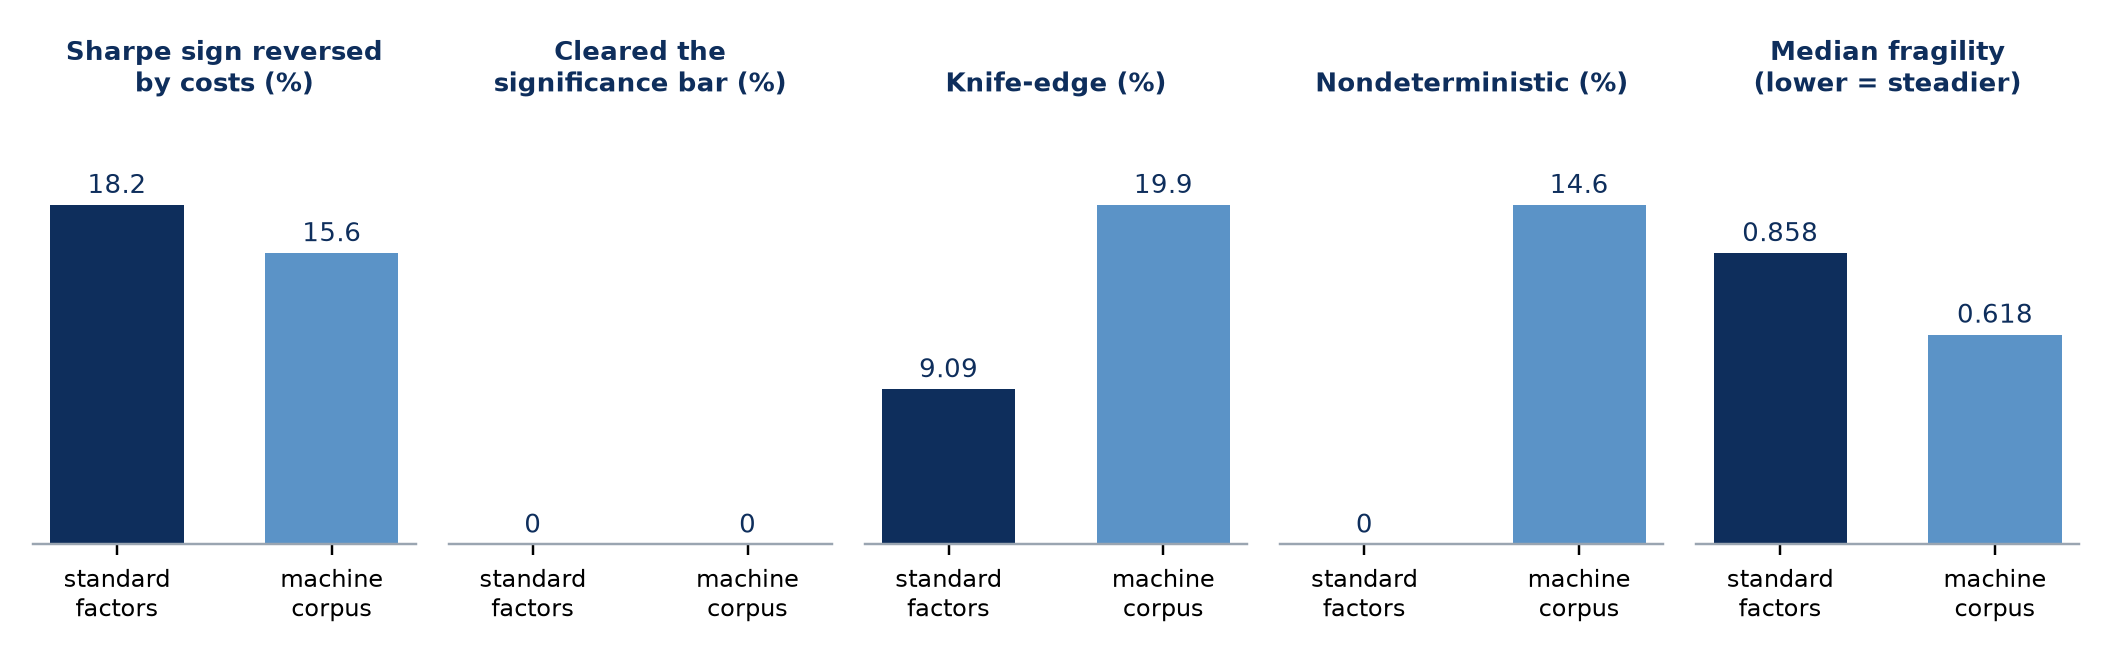
\includegraphics[width=\linewidth]{figures/fig_factors_vs_corpus.png}
\caption{The standard-factor arm against the machine-written corpus on five frozen tests. Each
panel has its own scale; the five quantities share no unit. $n=\sfN{}$ factors against corpora of
125--1{,}550 depending on the test.}
\label{fig:factorsvscorpus}
\end{figure}

\takeaway{Three tests separate the two arms and two do not. Machine-written strategies are
\emph{more} nondeterministic (\sfNondet{} of \sfN{} factors against 27 of 185) and land more static
leak flags. Costs and deflation treat both arms the same. \textbf{And fragility runs backwards} ---
the standard factors are \emph{more} fragile (\sfMedFrag{}) than the machine corpus (0.618),
because fragility scores consistency and the machine corpus is full of strategies that are
consistently near-flat. Paper 2 makes that argument in full.}

\begin{scopebox}
\textbf{These are \sfN{} strategies.} Every rate in Figure~\ref{fig:factorsvscorpus} computed on
the factor arm has a denominator of eleven, so a single strategy moves it by nine percentage
points. The arm is a control, not a sample --- it establishes that a verdict is \emph{not} specific
to machine authorship, and it cannot establish the size of any difference that remains.

\textbf{It is also not a ``human versus AI'' comparison and must not be read as one.} These
fixtures were hand-written for a different purpose, under no time limit, by an author who knew the
evaluation. The contrast the arm supports is \emph{published and long-standing} against
\emph{machine-written}, not \emph{human} against \emph{machine}.
\end{scopebox}

% =====================================================================================
\section{The auditor null}
\label{sec:null}

\begin{finding}
\tagindep\ \ Across \pgmNullCorpora{} independently generated corpora and all seven combinations
of the three auditor layers, \textbf{\pgmNullBeating{} of \pgmNullCombos{} configurations beat
random rejection at matched coverage} on out-of-sample data.
\end{finding}

\begin{figure}[t]\centering
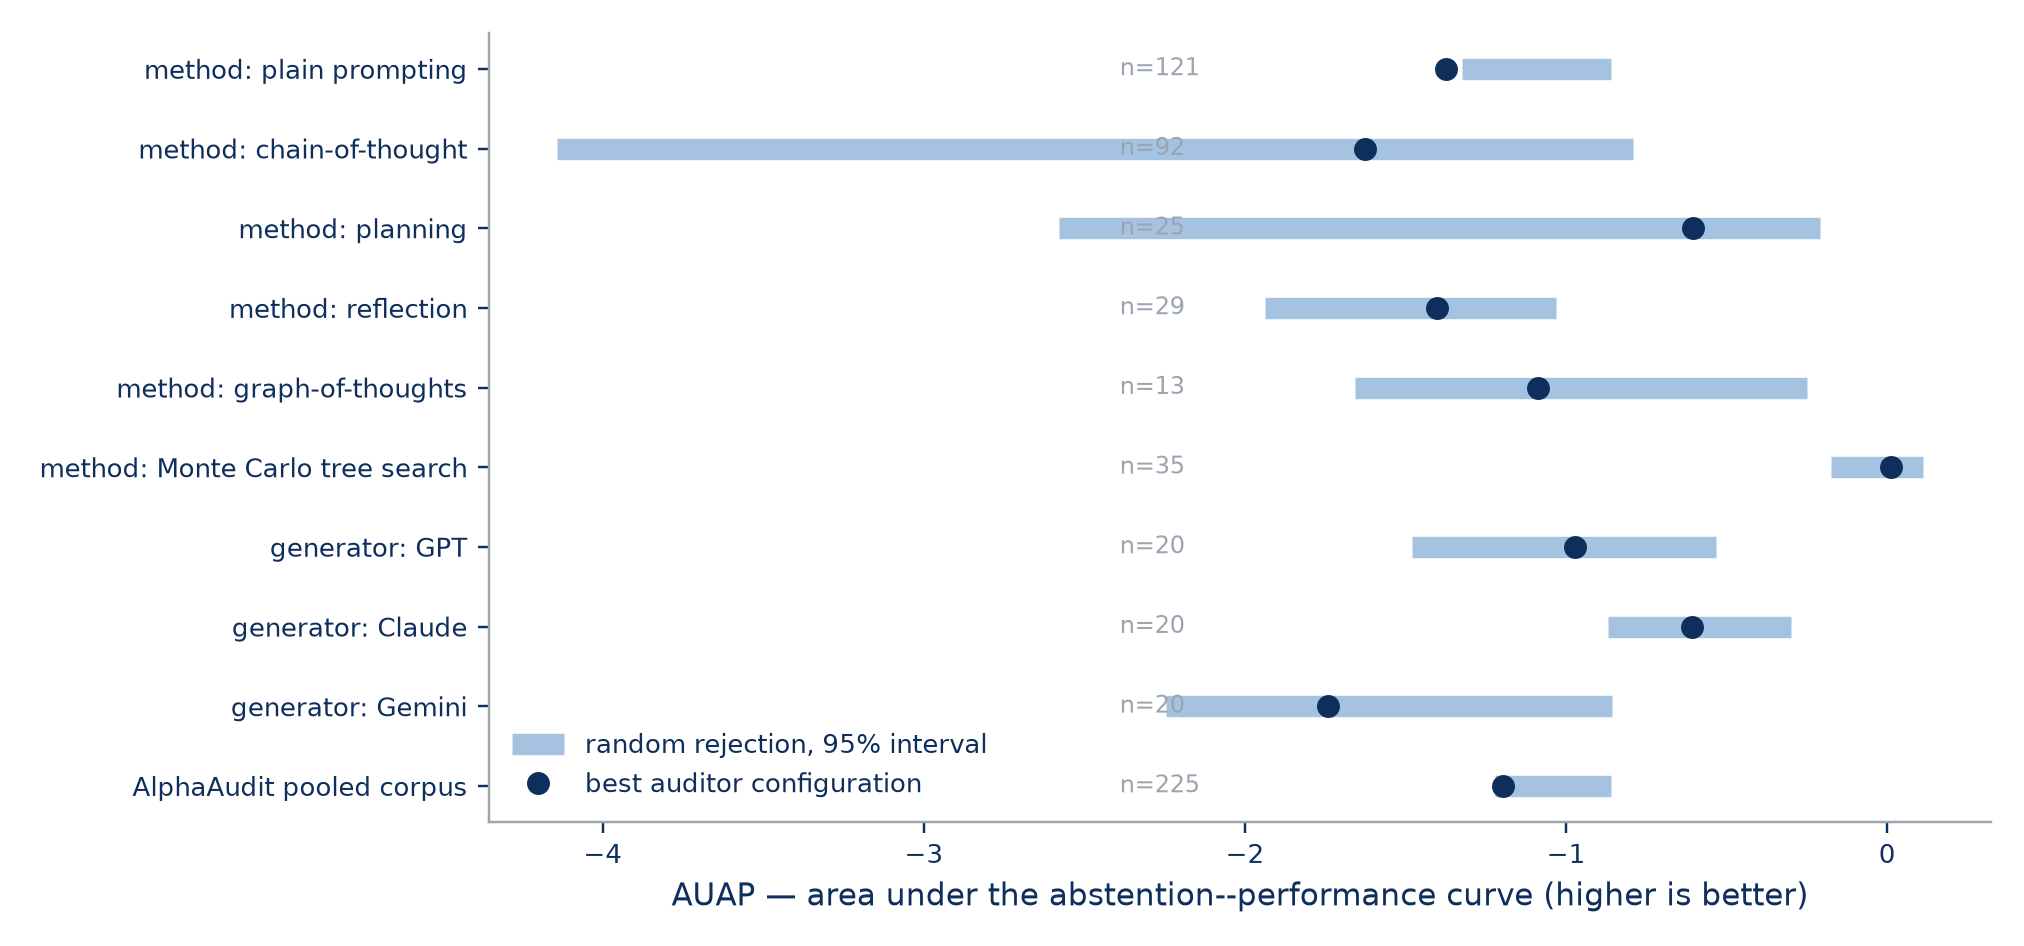
\includegraphics[width=\linewidth]{figures/fig_null_forest.png}
\caption{One row per corpus. The bar is that corpus's own random-rejection 95\% interval; the dot
is the best of seven auditor configurations. A working auditor's dot sits to the right of its bar.
None does. Sample sizes are printed per row and range from 13 to 225.}
\label{fig:null}
\end{figure}

\takeaway{The result does not depend on the generator, the generation method, or the corpus.
Every dot is inside or below its interval.}

Six of the ten corpora place the best configuration \emph{below} the random interval --- worse
than discarding at random. The pooled local corpus's best configuration is
$\aaLocalAuapBest{}$ against a random interval of
$[\aaLocalRandomLow{}, \aaLocalRandomHigh{}]$; the best frontier arm is
$\aaGvClaudeAuapBest{}$ against $[\aaGvClaudeRandomLow{}, \aaGvClaudeRandomHigh{}]$.
Across the frontier arms, \aaGvAuapBeats{} of \aaGvAuapCells{} configurations beat random.

\paragraph{The configuration that beat random in sample was the one that provably cannot.} Its
ranking signal is a monotone function of the quantity it was scored against, so its in-sample
advantage is arithmetic rather than information. Out of sample it fails with the rest.

\subsection{Two corrections, and what they did to the conclusion}
\label{sec:correction}

\begin{selfreport}[title={We found two defects in our own pipeline after first computing this null}]
The first was the entire cost implementation: the initial null was computed on a gross-of-costs
pipeline, which was found defective and rebuilt. The second was a sign error in the ranking
itself, which had been inverting the auditor's confidence order.

Both were repaired, the holdout was re-opened once for each under written prior authorisation, and
the null was recomputed. \textbf{The magnitudes moved. The conclusion did not.} No parameter,
threshold, prompt or model was changed after any holdout evaluation, and the diffs that produced
each correction are published rather than described.

We report this because a reader is entitled to ask whether a null that survived two corrections of
its own apparatus is a null or an artefact of a third defect not yet found. We cannot rule that
out. What we can do is publish the apparatus.
\end{selfreport}

\subsection{What the null does and does not establish}

\begin{scopebox}
\textbf{The null is confounded with corpus degeneracy and cannot separate ``the auditor is
uninformative'' from ``these corpora are too weak to test it''.}

The population being ranked is one in which \pgmLocalTrade\% of draws trade at all, nothing clears
deflation, and \aaLocalFlipsPct\% of the profitable reverse sign under costs. Asking an auditor to
rank that population for out-of-sample quality may be asking it to order noise. A stronger
generator would test the auditor properly --- and the frontier arms, which are a stronger
generator, produce the same null on a population that executes at 100\%. That narrows the
confound. It does not eliminate it, because those arms are \aaGvNLarge{} candidates each.
\end{scopebox}

% =====================================================================================
\section{What the auditor can and cannot detect}
\label{sec:limits-auditor}

Setting aside whether the ranking works, the layers have measurable and asymmetric competence.

\begin{center}\small
\begin{tabular}{p{0.28\linewidth}p{0.32\linewidth}p{0.32\linewidth}}
\toprule
\thead{Layer} & \thead{Detects, with evidence} & \thead{Blind to, with evidence} \\
\midrule
$A_{\mathrm{static}}$ &
All 3 leaky fixtures; 0 of 30 honest ones flagged; 4 leak classes observed in the wild &
\texttt{full\_sample\_statistic}: \textbf{0} findings in 1{,}550 sources, which we do not believe
(\S\ref{sec:leakclasses}). Unreachable code: flags a leak that never executes. \\
\midrule
$A_{\mathrm{stat}}$ &
Trial inflation, with a tamper-evident denominator; recovers the known result that a Sharpe of 2.0
from 200 dispersed trials is below chance &
\textbf{Everything, at this sample length.} It rejects published factors at their own trial count
(\S\ref{sec:factors}): \sfCleared{} of \sfN{} clear the bar, which requires an annualised Sharpe of
3.36 against a best observed of \sfBestNet{}. \\
\midrule
$A_{\mathrm{sem}}$ &
Rationale--implementation mismatch at $\kappa=0.589$ on 50 pre-labelled items; correctly passes a
leaky fixture whose rationale is honest &
\texttt{unfalsifiable\_mechanism}: 2 of 5 agreement. Whether its 154 rejections on the corpus are
the right ones is not established, since $\kappa$ was measured on a different population. \\
\bottomrule
\end{tabular}
\end{center}

\takeaway{The layers are not redundant --- the fixture that $A_{\mathrm{static}}$ catches is the
one $A_{\mathrm{sem}}$ correctly passes --- but neither is their union sufficient, and the
statistical layer is, on this window, a constant that we can now prove is a constant.}

% =====================================================================================
\section{Design flaws, mistakes, and things that did not work}
\label{sec:flaws}

A benchmark that reports only its successes is not measuring anything. Everything below is a defect
in our own apparatus or a result that failed, found by us, and none of it is elsewhere in the paper
only as a footnote. They are ordered by how much they cost.

\begin{table}[h]\centering\small
\caption{Every defect we found in our own pipeline, what it cost, and where it is discussed.}
\label{tab:flaws}
\begin{tabular}{p{0.30\linewidth}p{0.40\linewidth}p{0.22\linewidth}}
\toprule
\thead{Defect} & \thead{What it cost} & \thead{Where} \\
\midrule
Auditor's significance bar is unreachable &
Requires a 3.36 annualised Sharpe; nothing in the corpus or the factor arm approaches it. The
layer's verdict is uninformative and we cannot fix it without invalidating two holdout
evaluations. & \S\ref{sec:factors} \\
\midrule
The factor arm was never deflated &
The one population that made the layer's rejection rate interpretable was omitted for a year.
Found 2026-08-08. & \S\ref{sec:factors} \\
\midrule
Cost pipeline was gross-of-costs &
The entire first auditor null was computed on it. Rebuilt; holdout re-opened once under prior
authorisation. Conclusion unchanged. & \S\ref{sec:correction} \\
\midrule
Sign error in the ranking &
Inverted the auditor's confidence order for the whole first analysis. & \S\ref{sec:correction} \\
\midrule
Static layer's fixture score is training accuracy &
Recall was 1 of 3 until structural rules were added, then measured on the same three fixtures that
motivated them. The 100\% is not a test result. & \S\ref{sec:auditor} \\
\midrule
\texttt{full\_sample\_statistic} returns zero &
Not plausible in 1{,}550 candidates. Our own prompt almost certainly suppresses the class, so the
instrument is blind and the leak-class distribution describes this prompt. & \S\ref{sec:leakclasses} \\
\midrule
Trial ledger is 10 entries short &
1{,}877 recorded against 1{,}887 drawn. \textbf{Not repaired} --- an append-only ledger that gets
rewritten is not tamper-evident. Corrected at the point of use. & \S\ref{sec:selfreport-ledger} \\
\midrule
Flat candidates excluded, not ranked last &
A defensible choice that produces a higher abstention curve than the alternative. Stated, not
hidden. & \S\ref{sec:design} \\
\midrule
Survivors defined without the statistical layer &
The one place we chose the definition that yields a non-empty answer, because the honest one
yields nothing. & \S\ref{sec:design} \\
\midrule
Numbers predating the macro pipeline &
The cost and leak-class tables are transcribed rather than machine-inserted, so this paper's own
reproducibility guarantee has a hole in it. & \S\ref{sec:threats} \\
\bottomrule
\end{tabular}
\end{table}

\subsection{Results that failed}

\begin{itemize}
\item \textbf{The auditor does not beat random rejection}, on any of \pgmNullCorpora{} corpora or
  \pgmNullCombos{} configurations. This was the project's primary hypothesis.
\item \textbf{No scaffolded generation method beats plain prompting} at matched compute:
  \pgmScaffoldWins{} of \pgmScaffoldArms{}.
\item \textbf{Frontier models do not improve out-of-sample performance}, having entirely solved
  executability.
\item \textbf{The statistical layer discriminates nothing}, now demonstrated rather than suspected.
\item \textbf{One configuration beat random in sample} and was the one that provably cannot --- its
  ranking signal is a monotone function of the quantity it was scored against.
\end{itemize}

\begin{finding}
Five of the programme's headline hypotheses failed. We report all five, and the apparatus that
produced them is released so the failures can be contested rather than taken on trust.
\end{finding}

% =====================================================================================
\section{Threats to validity}
\label{sec:threats}

\paragraph{The prompt is a confound we cannot remove.} The prompt advises plain Python over polars
expression chains to raise executability, and that advice plausibly suppresses the
\texttt{full\_sample\_statistic} class to zero. Every leak-class distribution in this paper
describes this prompt.

\paragraph{One market, one period.} Indian equities, 2020--2024 development, 2025 holdout, the
hundred most liquid NSE names. Cost structure, retail participation and liquidity are specific to
that market; the execution-failure rates are specific to the libraries in the prompt.

\paragraph{Sample sizes differ by up to $40\times$ across arms.} \aaGvNLarge{} frontier draws
against \pgmPlainDraws{} for plain prompting; \pgmMctsDraws{} for tree search against
\pgmPlainDraws{}. Where a comparison is underpowered we compute the power and say so
(\S\ref{sec:methods}); we do not average across arms of different size, and no table in this paper
pools them.

\paragraph{The generator axis is not compute-matched, by construction.} Token spend for hosted
models is not comparable to local inference, so \S\ref{sec:frontier} reports rates only. No
sentence in it claims a frontier model is more \emph{efficient}.

\paragraph{The static layer's fixture score is closer to training accuracy than to a test.}
Stated in \S\ref{sec:auditor} where the number appears, not here.

\paragraph{The statistical layer's 100\% rejection rate is unresolved.} Stated in
\S\ref{sec:survives}. It is the threat we are least able to bound.

\paragraph{Numbers predating the macro pipeline are stated inline.} The local-corpus cost and
leak-class tables were computed before the generated-macro discipline was adopted, and are
transcribed rather than macro-substituted. They are regenerable from
\texttt{data/raw/} by documented commands, but they are not machine-inserted into this document,
and that is a real gap in the paper's own reproducibility guarantee.

\paragraph{Impact remains an assumption.} The square-root market-impact coefficient in the cost
model is uncalibrated. Paper 3 reports the measurement showing daily data cannot calibrate it, so
this is a permanent property of the apparatus rather than a to-do.

% =====================================================================================
\section{What this tells us about AI-driven research}
\label{sec:meaning}

\begin{finding}
\textbf{Can AI write code? Yes, increasingly and now essentially completely. Can AI generate
statistically credible quantitative research? On this apparatus, much less clearly --- and the
first capability improving did not cause the second to.}
\end{finding}

Three claims, at three different scopes, which the rest of this section keeps separate because
collapsing them is the error the programme was built to avoid.

\paragraph{Generator-independent \tagindep} The auditor null holds on all
\pgmNullCorpora{} corpora, produced by four generators and six methods. Nothing clears deflation
on any arm. Costs reverse signs on every arm. These are the claims that survive a change of
generator, and they are the ones that license the apparatus being used by anyone else.

\paragraph{Generator-specific \taglocal\ \tagfrontier} The execution barrier is a property of the
local 7B, not of machine-written strategies: \pgmLocalTrade\% against 100\%. Any paper reporting
execution rates for one model is reporting that model. Our own paper 1 result, published before
the frontier arms existed, was such a claim, and this section is where we say so.

\paragraph{Method-specific \tagmethod} Scaffolding buys candidates, not quality, at equal budget:
\pgmScaffoldWins{} of \pgmScaffoldArms{} arms beat their control. This is the claim most likely to
generalise beyond finance, because it is a claim about compute accounting rather than about
markets.

\subsection{The one recommendation we are willing to make}

If you evaluate a machine-written quantitative finding, the ordering that matters is: \emph{does
it run}, then \emph{does it survive costs}, then \emph{does it survive the number of things you
tried}, then \emph{does it survive data you have never seen}. Most published pipelines measure the
first and report the fourth. The attrition between them, on this corpus, is total.

% =====================================================================================
\section{The AlphaAudit benchmark}
\label{sec:benchmark}

Frozen and released at \repo:

\begin{itemize}
\item \textbf{Environment.} Survivorship-free point-in-time universe, verified cost model,
  raising point-in-time engine, purged cross-validation with embargo.
\item \textbf{Fixtures.} 3 deliberately-leaky and 30 honest strategies, permanent assets.
\item \textbf{Corpus.} \pgmParadigmDraws{} machine-written candidates across
  \pgmParadigmArms{} generation methods, plus \aaGvTotal{} frontier candidates and the
  \aaLocalDraws{}-draw local corpus, each with audit verdicts, backtests, and holdout results
  where applicable.
\item \textbf{Protocol.} The frozen task specification and its digest, the abstention--performance
  harness, the random-rejection baseline, and the trial ledger with its verification.
\item \textbf{Every number.} \texttt{RESULTS.md} per benchmark, and the generated macro files this
  paper is built from. If this paper and the repository disagree, the repository is right.
\end{itemize}

A stronger auditor can be scored against exactly this apparatus and contest the null directly.
That is the point of releasing an environment whose reference implementation failed.

% =====================================================================================
\section{Conclusion}

We built an environment in which a machine-written trading strategy can be scored for validity
rather than for plausibility, and we ran four generators and six generation methods through it
without changing it between arms.

The local model's strategies fail as programs, not as research: 100\% produce conforming code and
\pgmLocalTrade\% produce a strategy that trades. Frontier models remove that barrier entirely, at
100\%. \textbf{They remove nothing else.} Zero of \aaGvTotal{} frontier candidates clear
deflation; \aaGvFlipsTotal{} reverse sign under costs; every arm's median holdout Sharpe is
negative. More elaborate generation methods lose to plain prompting at every matched token budget
we measured. And across \pgmNullCorpora{} corpora, \pgmNullBeating{} of \pgmNullCombos{} auditor
configurations beat random rejection out of sample.

\begin{finding}
\textbf{Better code did not mean better quantitative research.} That is one measurement, on one
market, on one apparatus, with the confounds named in \S\ref{sec:threats}. It is also the
measurement the field is currently not making, and the apparatus for making it is now public.
\end{finding}

\subsection*{Where this leaves us}
\addcontentsline{toc}{subsection}{Where this leaves us}

This paper asked whether a machine-written strategy is \emph{real}. For most of the corpus the
answer was no, and the survivors it hands forward --- defined by
$A_{\mathrm{static}} \wedge A_{\mathrm{sem}}$, since the statistical layer leaves nothing --- are
a small set of low-turnover strategies that survived costs and one holdout year.

Surviving one history is a weak claim. The 2020--2024 development window contains one pandemic
crash, one full rate cycle and one structural liquidity shift; a strategy that survived it
survived a single sequence of events, and the number of independent regime observations available
is very small. \textbf{The next question is therefore not whether these strategies are real, but
when they break} --- and answering it requires plausible histories that did not happen, because
history did not supply enough of them.

That is paper 2, \textbf{RegimeStress}.

% =====================================================================================
\small
\begin{thebibliography}{99}

\bibitem[Almgren et al.(2005)]{almgren2005}
Almgren, R., Thum, C., Hauptmann, E., and Li, H. (2005).
Direct estimation of equity market impact. \emph{Risk}, 18(7), 58--62.

\bibitem[Bailey and L\'opez de Prado(2014)]{bailey2014}
Bailey, D. H., and L\'opez de Prado, M. (2014).
The Deflated Sharpe Ratio: Correcting for selection bias, backtest overfitting, and
non-normality. \emph{The Journal of Portfolio Management}, 40(5), 94--107.

\bibitem[Bailey et al.(2017)]{bailey2017}
Bailey, D. H., Borwein, J., L\'opez de Prado, M., and Zhu, Q. J. (2017).
The Probability of Backtest Overfitting. \emph{Journal of Computational Finance}, 20(4),
39--69.

\bibitem[Besta et al.(2024)]{besta2024}
Besta, M., Blach, N., Kubicek, A., et al. (2024).
Graph of Thoughts: Solving Elaborate Problems with Large Language Models.
\emph{Proceedings of the AAAI Conference on Artificial Intelligence}, 38(16), 17682--17690.

\bibitem[Chen et al.(2021)]{chen2021}
Chen, M., Tworek, J., Jun, H., et al. (2021).
Evaluating Large Language Models Trained on Code. \emph{arXiv:2107.03374}.

\bibitem[Cohen(1960)]{cohen1960}
Cohen, J. (1960). A coefficient of agreement for nominal scales.
\emph{Educational and Psychological Measurement}, 20(1), 37--46.

\bibitem[El-Yaniv and Wiener(2010)]{elyaniv2010}
El-Yaniv, R., and Wiener, Y. (2010). On the foundations of noise-free selective
classification. \emph{Journal of Machine Learning Research}, 11, 1605--1641.

\bibitem[Frazzini et al.(2018)]{frazzini2018}
Frazzini, A., Israel, R., and Moskowitz, T. J. (2018).
Trading costs. \emph{SSRN Working Paper 3229719}.

\bibitem[Geifman and El-Yaniv(2017)]{geifman2017}
Geifman, Y., and El-Yaniv, R. (2017). Selective classification for deep neural networks.
\emph{Advances in Neural Information Processing Systems}, 30.

\bibitem[Harvey et al.(2016)]{harvey2016}
Harvey, C. R., Liu, Y., and Zhu, H. (2016).
$\ldots$ and the Cross-Section of Expected Returns.
\emph{The Review of Financial Studies}, 29(1), 5--68.

\bibitem[Jegadeesh and Titman(1993)]{jegadeesh1993}
Jegadeesh, N., and Titman, S. (1993). Returns to buying winners and selling losers:
Implications for stock market efficiency. \emph{The Journal of Finance}, 48(1), 65--91.

\bibitem[Landis and Koch(1977)]{landis1977}
Landis, J. R., and Koch, G. G. (1977). The measurement of observer agreement for categorical
data. \emph{Biometrics}, 33(1), 159--174.

\bibitem[L\'opez de Prado(2018)]{lopezdeprado2018}
L\'opez de Prado, M. (2018). \emph{Advances in Financial Machine Learning}. Wiley.

\bibitem[Novy-Marx and Velikov(2016)]{novymarx2016}
Novy-Marx, R., and Velikov, M. (2016). A taxonomy of anomalies and their trading costs.
\emph{The Review of Financial Studies}, 29(1), 104--147.

\bibitem[Shinn et al.(2023)]{shinn2023}
Shinn, N., Cassano, F., Gopinath, A., Narasimhan, K., and Yao, S. (2023).
Reflexion: Language Agents with Verbal Reinforcement Learning.
\emph{Advances in Neural Information Processing Systems}, 36.

\bibitem[Wei et al.(2022)]{wei2022}
Wei, J., Wang, X., Schuurmans, D., et al. (2022).
Chain-of-Thought Prompting Elicits Reasoning in Large Language Models.
\emph{Advances in Neural Information Processing Systems}, 35, 24824--24837.

\bibitem[Wu et al.(2023)]{wu2023}
Wu, S., Irsoy, O., Lu, S., et al. (2023).
BloombergGPT: A Large Language Model for Finance. \emph{arXiv:2303.17564}.

\bibitem[Yao et al.(2023)]{yao2023}
Yao, S., Yu, D., Zhao, J., et al. (2023).
Tree of Thoughts: Deliberate Problem Solving with Large Language Models.
\emph{Advances in Neural Information Processing Systems}, 36.

\end{thebibliography}

\end{document}
